\chapter{DISEÑO ELECTRÓNICO DEL SISTEMA}\label{cap:diseno-electronico}
\listasdecapitulo{4}

El diseño electrónico parte de las funciones que el módulo debe cumplir y de los requerimientos definidos
en capítulos previos, no de la mera disponibilidad comercial de los componentes. Se mantiene la premisa
arquitectónica del sistema: el controlador semafórico existente conserva la autoridad final de actuación y
el módulo electrónico se limita a sensar, procesar localmente y recomendar. En consecuencia, cada selección
se justifica por su aporte a la disponibilidad del lazo local, su seguridad eléctrica y su trazabilidad
frente a los requisitos. La verificación mecánica de los actuadores y la disposición física de los
componentes en el gabinete se desarrollan en el Capítulo~\ref{cap:diseno-mecanico}.

\section{Criterios de selección y relación con requerimientos}\label{sec:criterios-electronicos}

La selección electrónica se realiza por función y requerimiento. Para cada elemento se identifica la
alternativa considerada, el criterio de elección, su limitación principal y el modo de falla que debe
tratarse en la integración. La Tabla~\ref{tab:seleccion-electronica} resume esta trazabilidad
función--alternativa--criterio--selección--justificación--limitación--requisito, que sirve de hilo conductor
para el resto del capítulo.

\begin{landscape}
\begin{table}[htbp]
  \centering
  \caption{Selección trazable de componentes electrónicos.}
  \label{tab:seleccion-electronica}
  \footnotesize
  \begin{tabular}{@{}p{2.8cm}p{3.6cm}p{3.4cm}p{2.9cm}p{4.6cm}p{2.1cm}@{}}
    \toprule
    \textbf{Función/componente} & \textbf{Alternativas} & \textbf{Criterios} & \textbf{Selección de diseño} & \textbf{Justificación, limitación y modo de falla} & \textbf{Requisito}\\
    \midrule
    Sensado de tráfico & Cámara RGB, radar, lazo, LiDAR & Información obtenida, obra civil, costo, mantenimiento & Cámara exterior & Entrega múltiples variables sin intervenir el pavimento; sensible a oclusión e iluminación. Ante baja calidad debe inhibirse la adaptación. & R-F01, R-C04\\
    Procesamiento local & MCU, SBC, mini PC industrial, nube & Capacidad de visión, latencia, consumo, costo & SBC/edge computer & Permite visión y control local; requiere gestión térmica, almacenamiento robusto y watchdog. & R-C01, R-ELEC03\\
    Comunicación & Ethernet, Wi-Fi, 4G/LTE, fibra & Cobertura, independencia, costo y disponibilidad & 4G/LTE con Ethernet disponible & Facilita el despliegue; la pérdida de enlace no debe detener el control local. & R-COM01, R-VAL03\\
    Monitoreo eléctrico & Shunt, efecto Hall, medidor digital & Aislamiento, rango, precisión, interfaz & Sensor aislado tipo Hall & Permite diagnóstico; una medición fuera de rango genera alerta, no una decisión de fase. & R-ELEC03\\
    Fuente principal & Fuente abierta, industrial DIN, ATX & Protección, eficiencia, temperatura, mantenibilidad & Fuente industrial AC/DC & Adecuada para operación continua; se dimensiona con margen y coordinación de protecciones. & R-ELEC01\\
    Conversión DC/DC & Lineal, buck comercial, módulo industrial & Eficiencia, ruido, rango y protección & Convertidores buck regulados & Reduce pérdidas; requiere filtrado y separación de cargas sensibles y motores. & R-ELEC01, R-ELEC03\\
    Respaldo & Sin respaldo, power bank, UPS, batería DC & Autonomía, seguridad, mantenimiento & UPS dimensionado & Mantiene registro y apagado controlado; autonomía verificada con el perfil de carga real. & R-ELEC02\\
    Interfaz con controlador & Relé directo, GPIO, protocolo estándar, API & Seguridad, aislamiento, compatibilidad, autoridad final & Interfaz aislada; NTCIP cuando sea compatible & No se autoriza mando directo de lámparas. Falla o incompatibilidad implica retorno a solo supervisión. & R-C02, R-COM02\\
    \bottomrule
  \end{tabular}
  \fuente{Elaboración propia.}
\end{table}
\end{landscape}

\section{Componentes electrónicos}\label{sec:componentes-electronicos}

\subsection{Sensores}\label{subsec:sensores}

\subsubsection{Sensor de temperatura}

Para el monitoreo térmico del interior del gabinete se evaluaron el DS18B20, el DHT22 y el LM35,
priorizando escalabilidad, inmunidad al ruido y simplicidad de integración. Se selecciona el sensor digital
\textbf{DS18B20}, que entrega lecturas en un rango de $-55$\,°C a $+125$\,°C con resolución configurable de 9
a 12 bits y precisión de \ensuremath{\pm}0.5\,°C en el rango operativo típico ($-10$\,°C a $+85$\,°C),
suficiente para detectar sobrecalentamientos. Su protocolo OneWire permite conectar varios sensores a un
único pin GPIO mediante un código único de 64 bits por dispositivo, evita el uso de un ADC externo y, al ser
digital, ofrece inmunidad al ruido electromagnético generado por relés y contactores. Como única
consideración de integración, requiere una resistencia pull-up de 4.7\,k\ensuremath{\Omega} entre la línea
de datos y la alimentación. La comparación detallada de alternativas se incluye en el Anexo.

\begin{figure}[H]
  \centering
  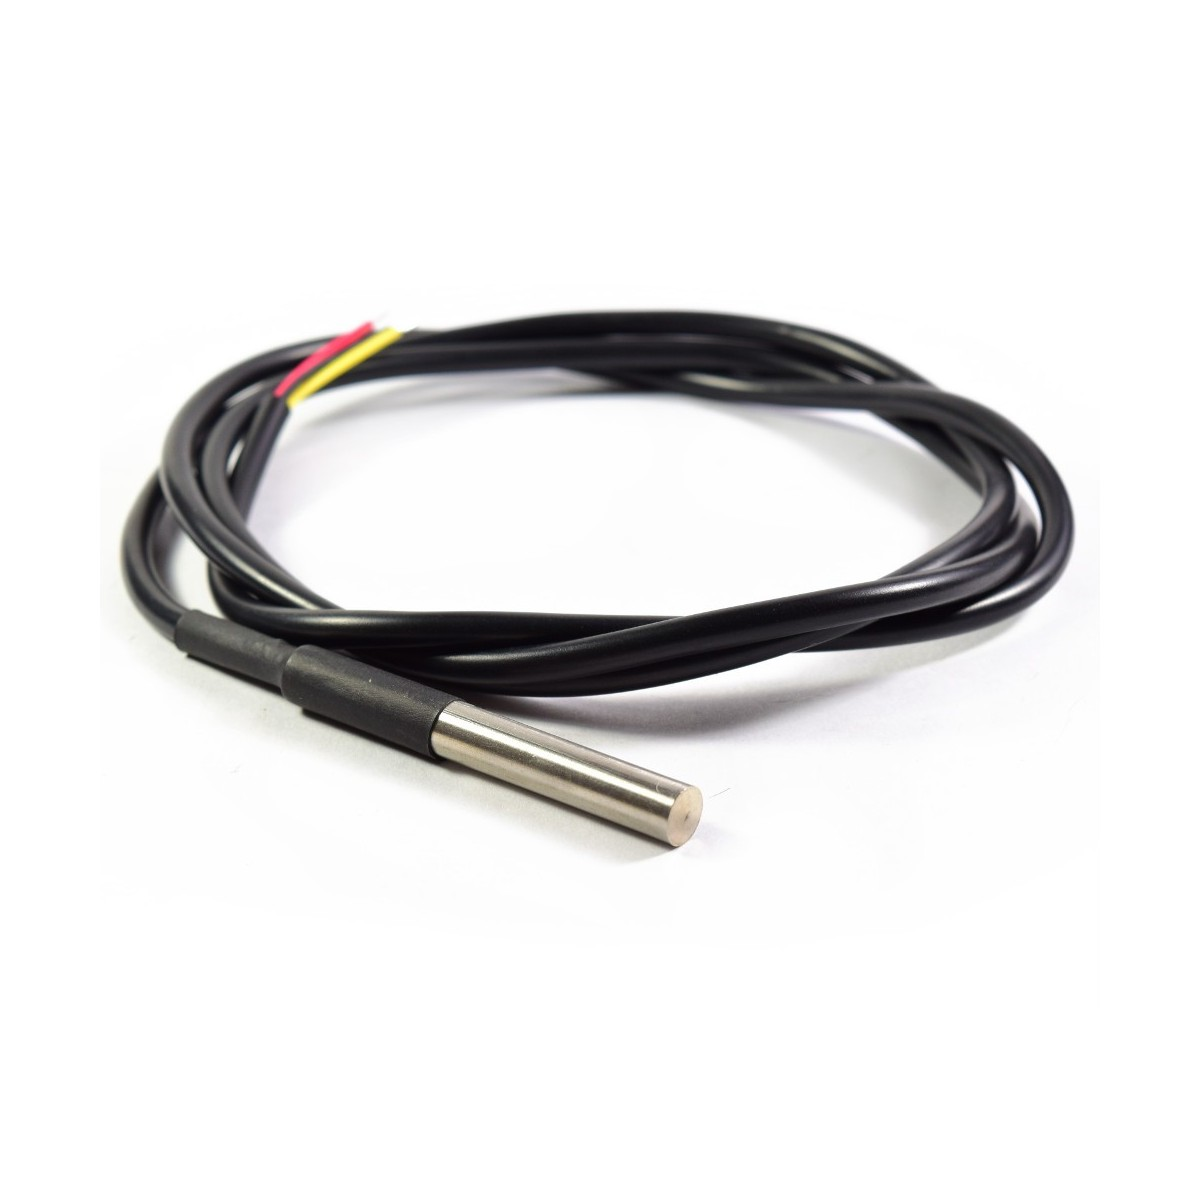
\includegraphics[width=0.55\linewidth,keepaspectratio]{media/image89.png}
  \caption{Sensor digital de temperatura DS18B20.}
  \label{fig:ds18b20}
  \fuente{Adaptado de la hoja de datos del fabricante.}
\end{figure}

\subsubsection{Sensor de corriente}

Para medir la corriente del sistema se compararon el WCS1600 (efecto Hall), el ACS712 y un transformador de
corriente (CT). Se selecciona el \textbf{WCS1600}, que mide corriente DC y AC sin contacto directo con el
conductor (hasta \ensuremath{\pm}100\,A DC y 70\,A RMS AC), rango que cubre holgadamente las cargas del
sistema. Su principal ventaja es el aislamiento galvánico inherente al efecto Hall, que protege a la unidad
de control ante fallas de la instalación y no introduce pérdidas resistivas en el circuito de potencia, a
diferencia de un shunt. Dado que la Raspberry Pi 5 carece de ADC integrado, la salida analógica del sensor
(0.3--4.7\,V, con 2.5\,V para corriente nula) se digitaliza con el ADC \textbf{MCP3008} de 10 bits por bus
SPI; la conversión a corriente se realiza con $I = (V_{out}-2.5)\times 45.4545$. Para lecturas correctas, un
solo conductor debe atravesar por completo el orificio del sensor.

\begin{figure}[H]
  \centering
  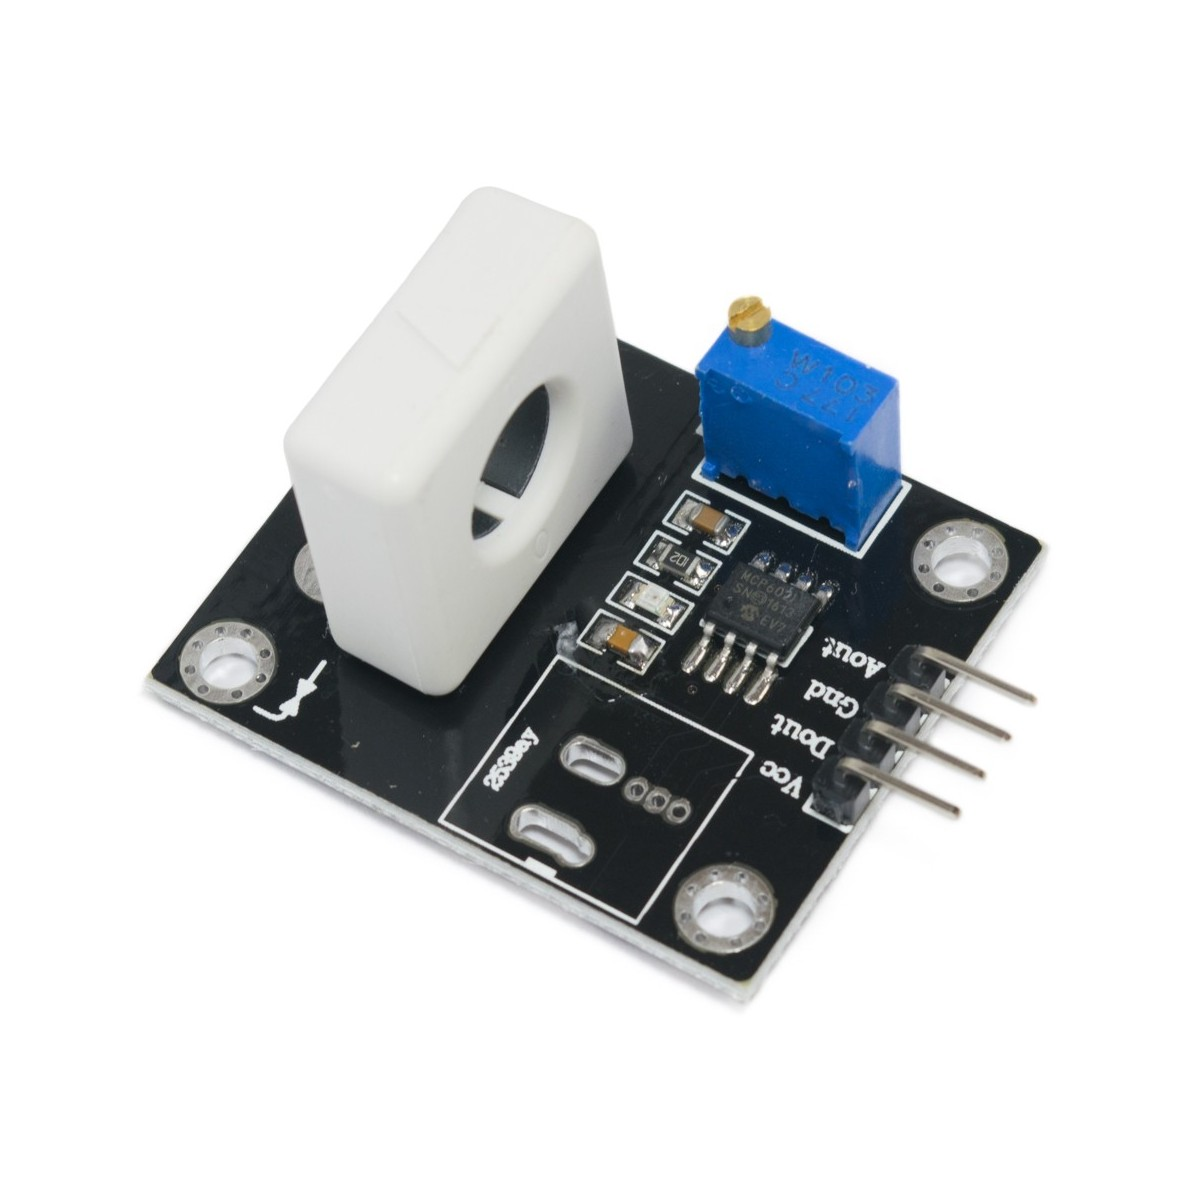
\includegraphics[width=0.55\linewidth,keepaspectratio]{media/image75.png}
  \caption{Módulo sensor de corriente de efecto Hall WCS1600.}
  \label{fig:wcs1600}
  \fuente{Adaptado de la hoja de datos del fabricante.}
\end{figure}

\subsubsection{Sensor de presencia}

Para detectar la aproximación de vehículos al gabinete se evaluaron el ultrasónico URM06, el HC-SR04 y
sensores infrarrojos. Se selecciona el \textbf{URM06} con interfaz UART, con rango de 0.2 a 10\,m y haz
estrecho de aproximadamente 15°, que concentra la energía acústica y reduce las detecciones falsas por
reflexiones laterales propias del HC-SR04. Frente a los sensores infrarrojos, presenta inmunidad a la luz
solar directa; la interfaz UART permite enviar comandos y recibir distancias en formato digital sin
electrónica adicional. Su limitación es la atenuación del eco ante superficies absorbentes del sonido, que
puede reducir el alcance efectivo. El detalle comparativo se traslada al Anexo.

\begin{figure}[H]
  \centering
  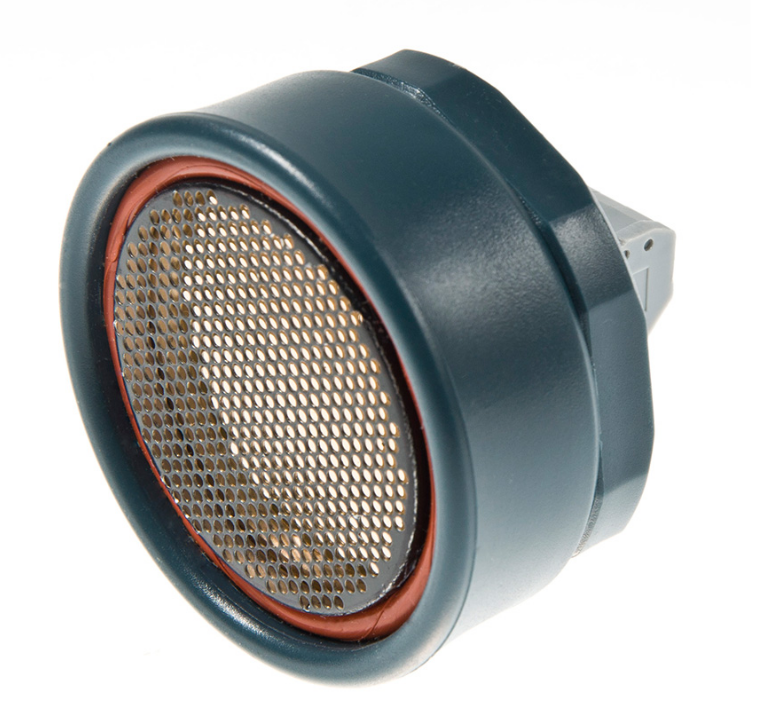
\includegraphics[width=0.55\linewidth,keepaspectratio]{media/image150.png}
  \caption{Sensor ultrasónico de presencia URM06 con interfaz UART.}
  \label{fig:urm06}
  \fuente{Adaptado de la hoja de datos del fabricante.}
\end{figure}

\subsubsection{Cámara de visión por computadora}

El sensor principal de tráfico es una \textbf{cámara tipo domo Hikvision DS-2CE57H0T-VPITF}, única cámara
del sistema, destinada a la detección y el seguimiento de vehículos mediante visión por computadora (modelos
tipo YOLO ejecutados en la unidad de control). Se comparó contra configuraciones PTZ, bullet y otras
cámaras, prefiriéndose el domo fijo por su robustez ambiental y su discreción. Entrega 5\,MP
($2560\times1944$) a 20\,fps, tasa suficiente para el seguimiento vehicular sin la carga computacional de
30 o 60\,fps, e incorpora iluminación infrarroja EXIR 2.0 con alcance de unos 20\,m para operación nocturna.
La carcasa IP67/IK10 soporta polvo, lluvia, vandalismo e impactos de hasta 20\,J, y la lente de 2.8\,mm
cubre unos 103° horizontales, abarcando intersecciones de hasta tres carriles por sentido con una sola
cámara.

La cámara entrega video HD-TVI sobre cable coaxial, formato no compatible directamente con la Raspberry Pi.
Para resolverlo se emplea un \textbf{convertidor de video 4-en-1 (AHD/CVBS/CVI/TVI a USB)}, que la presenta
al sistema operativo como una webcam USB estándar accesible mediante OpenCV, V4L2 o FFmpeg. Esta solución
sobre coaxial admite tendidos largos (hasta cientos de metros) con buena inmunidad electromagnética, frente
a los pocos metros de las interfaces CSI, reservadas como expansión futura para cámaras de corto alcance.

\begin{figure}[H]
  \centering
  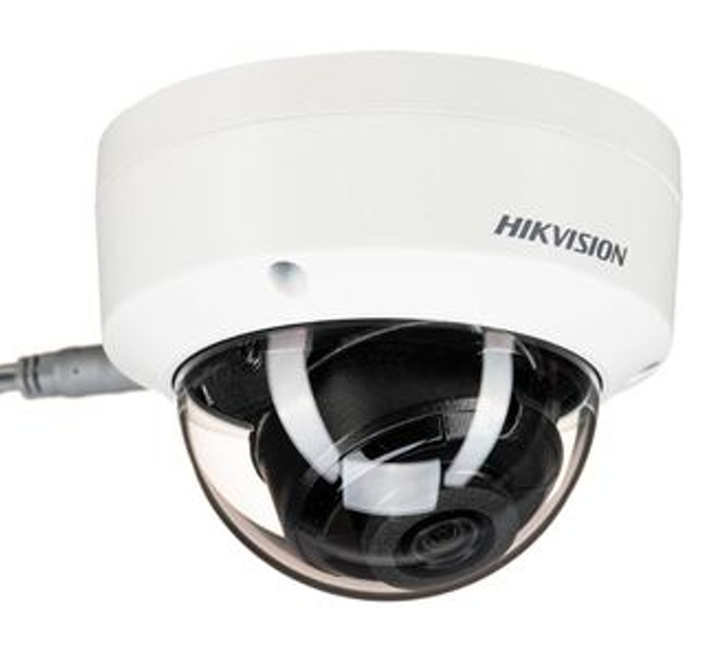
\includegraphics[width=0.5\linewidth,keepaspectratio]{media/image110.png}
  \caption{Cámara domo Hikvision DS-2CE57H0T-VPITF empleada para la visión por computadora.}
  \label{fig:camara}
  \fuente{Adaptado de la hoja de datos del fabricante.}
\end{figure}

\begin{figure}[H]
  \centering
  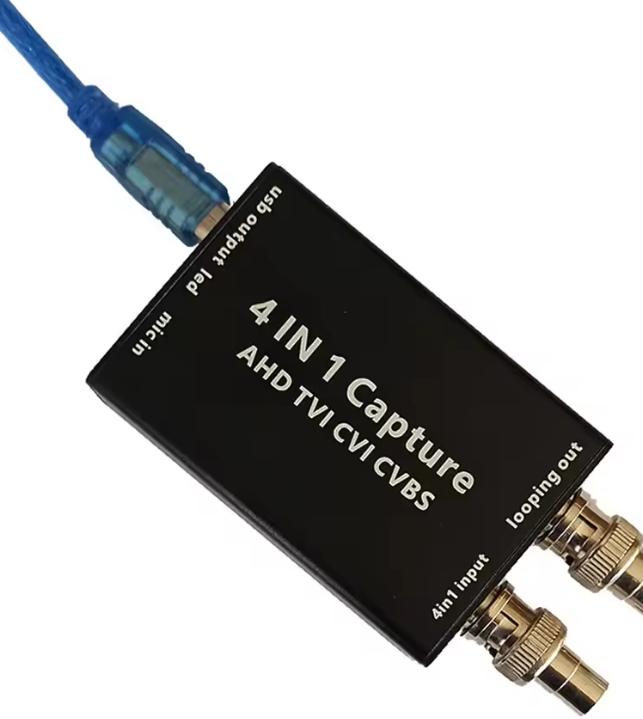
\includegraphics[width=0.5\linewidth,keepaspectratio]{media/image85.png}
  \caption{Convertidor de video 4-en-1 AHD/CVBS/CVI/TVI a USB para la interfaz con la unidad de control.}
  \label{fig:conv-video}
  \fuente{Adaptado de la hoja de datos del fabricante.}
\end{figure}

\subsection{Actuador de posicionamiento de cámara}\label{subsec:actuador}

El sistema de posicionamiento angular de la cámara (aro giratorio accionado por biela-manivela, detallado en el
Capítulo~\ref{cap:diseno-mecanico}) requiere un actuador con posicionamiento preciso y repetible y torque
suficiente frente a vibraciones. Se evaluaron motor DC, servomotor y motor paso a paso,
y se selecciona el \textbf{motor paso a paso NEMA 23} (modelo 57H1876-420-8-21B, bipolar de 4 hilos,
200 pasos por revolución), alimentado a \textbf{24\,V DC}, con \textbf{torque máximo de 1.8\,N\ensuremath{\cdot}m}
(18.4\,kg\ensuremath{\cdot}cm) y corriente nominal de 4.2\,A por fase. La elección frente al servomotor o al
motor DC con encoder se fundamenta en el control de posición en lazo abierto, sin realimentación compleja, y
en un torque holgado para mover la cámara domo y su soporte. La \textit{verificación del torque requerido}
(estático, dinámico y márgenes de seguridad mecánicos) se desarrolla en el
Capítulo~\ref{cap:diseno-mecanico} para evitar duplicidad; en este capítulo se documenta únicamente la
selección eléctrica del actuador y su cadena de control.

\begin{figure}[H]
  \centering
  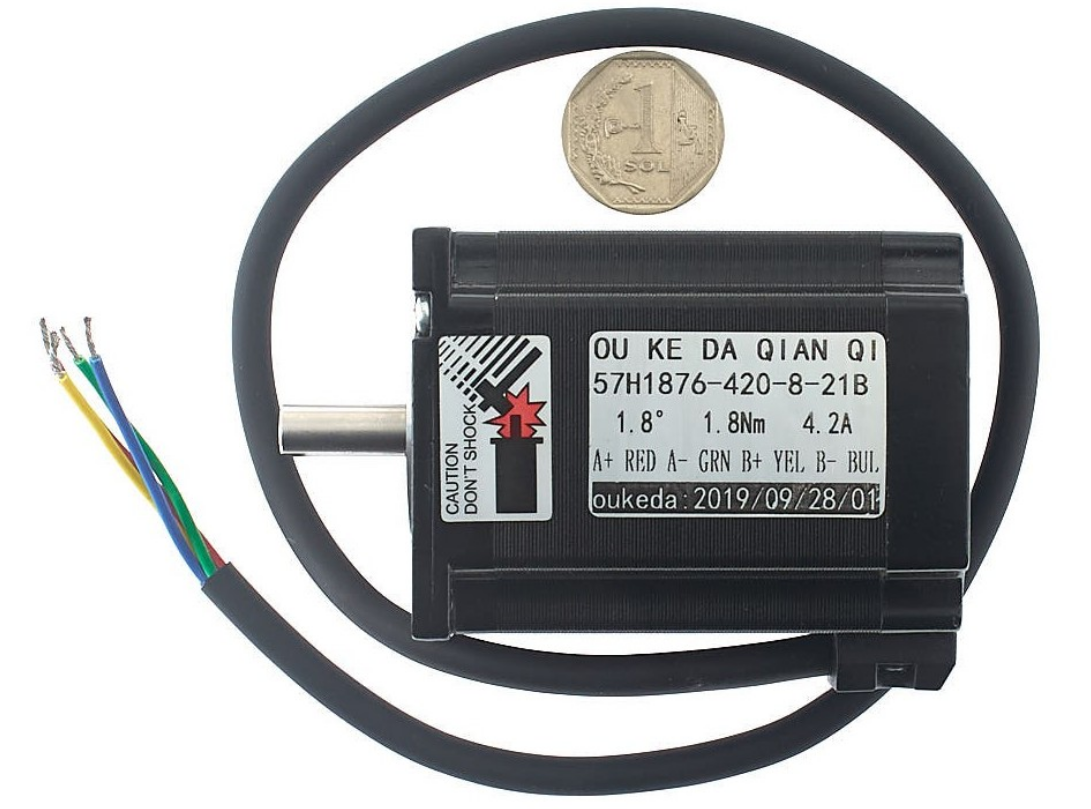
\includegraphics[width=0.5\linewidth,keepaspectratio]{media/image157.png}
  \caption{Motor paso a paso NEMA 23 seleccionado como actuador de la cámara.}
  \label{fig:nema23}
  \fuente{Adaptado de la hoja de datos del fabricante.}
\end{figure}

\subsubsection{Driver del motor}

El motor paso a paso bipolar se gobierna con el driver digital \textbf{DM542T}, basado en DSP, que genera la
conmutación secuencial de corriente en las bobinas y aporta protecciones eléctricas. Admite micropaso (hasta
15 resoluciones); una configuración de 1600 pasos/revolución (1/8 de paso) otorga 0.225° de resolución
angular. Su rango de alimentación de 18--50\,V DC y de corriente ajustable de 1.0 a 4.5\,A por DIP-switch se
adecua al motor seleccionado (4.2\,A nominales). El driver se comanda con tres señales digitales: PUL
(pulso), DIR (dirección) y ENA (habilitación), esta última útil para desenergizar las bobinas y reducir
consumo y calentamiento cuando no se requiere mantener posición.

\begin{figure}[H]
  \centering
  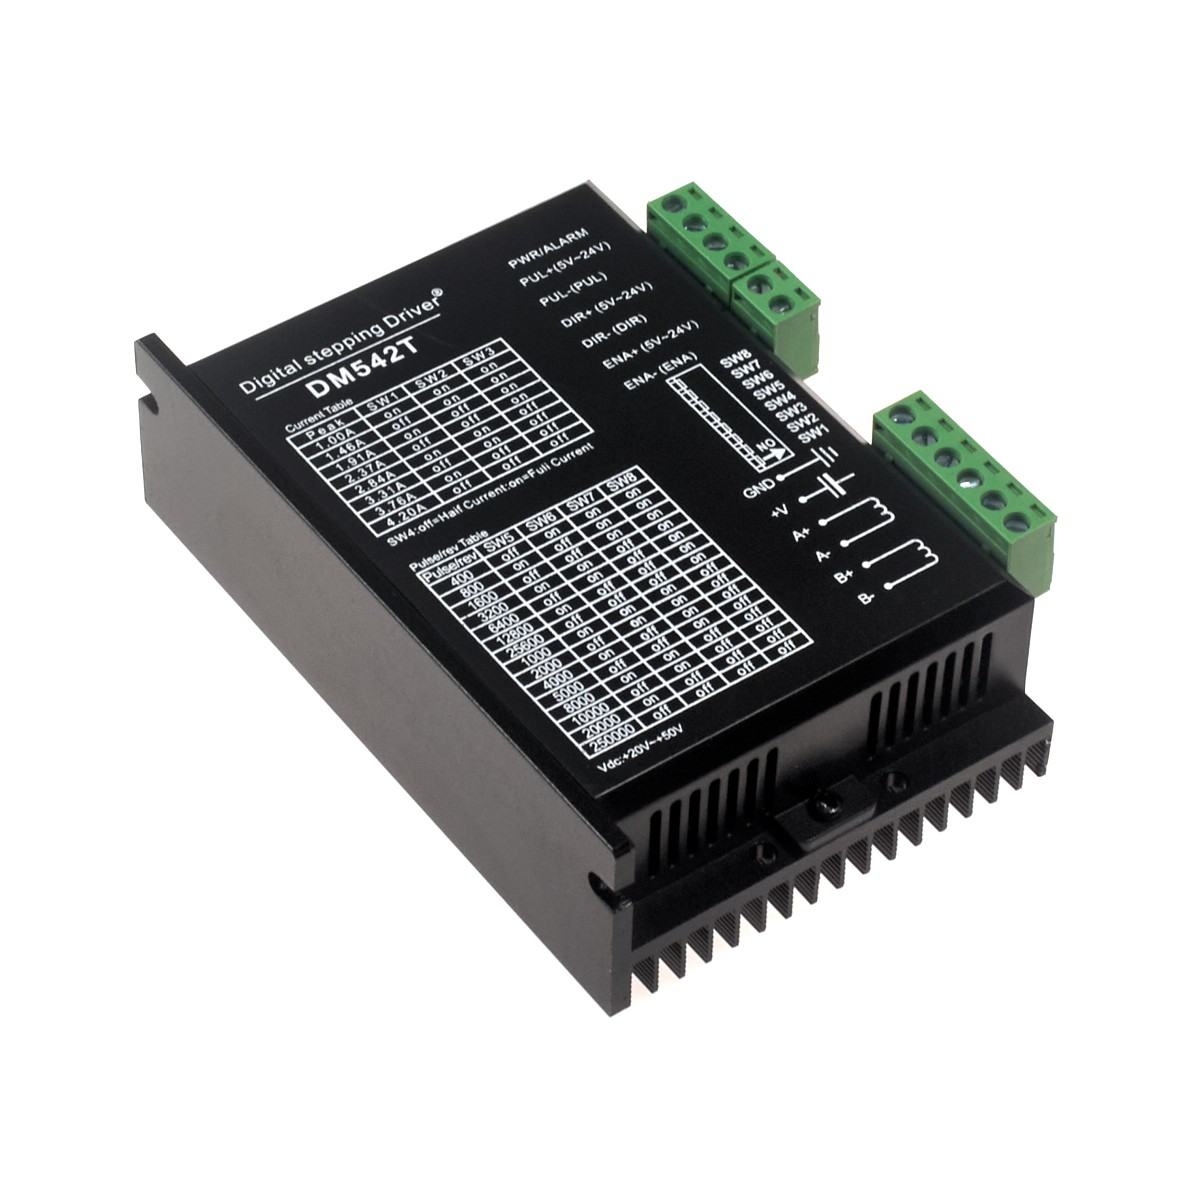
\includegraphics[width=0.5\linewidth,keepaspectratio]{media/image153.png}
  \caption{Driver digital DM542T para el motor paso a paso.}
  \label{fig:dm542t}
  \fuente{Adaptado de la hoja de datos del fabricante.}
\end{figure}

\subsubsection{Convertidor de nivel lógico}

Las señales de control salen de la Raspberry Pi a 3.3\,V y el driver opera a 5\,V. Para adaptar ambos niveles
se utiliza un convertidor bidireccional de 8 canales basado en el chip \textbf{TXS0108E}, que detecta la
dirección de la señal y traduce el voltaje automáticamente. Aunque las señales de control del motor son
unidireccionales, la bidireccionalidad deja margen para futuras señales de retorno, como límites de carrera
o alarmas.

\begin{figure}[H]
  \centering
  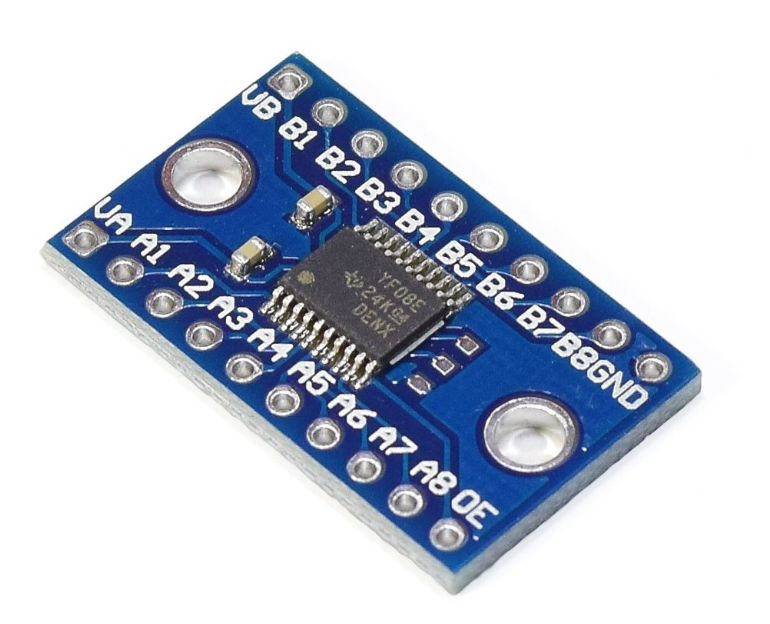
\includegraphics[width=0.5\linewidth,keepaspectratio]{media/image20.png}
  \caption{Convertidor de nivel lógico bidireccional de 8 canales 5\,V/3.3\,V.}
  \label{fig:level-shifter}
  \fuente{Adaptado de la hoja de datos del fabricante.}
\end{figure}

\paragraph{Robustez para entorno vial (criterios de diseño a confirmar en prototipo).} El entorno de
instalación es eléctricamente ruidoso (conmutación de contactores, transitorios de red y EMI de la cámara),
por lo que la cadena de control del motor admite mejoras de robustez que se dejan planteadas como criterio de
diseño y deben validarse en la etapa de prototipo. En primer lugar, el convertidor TXS0108E adapta niveles de
voltaje pero no proporciona aislamiento galvánico; para una versión de campo se recomienda intercalar
optoacopladores rápidos —o un \emph{driver} con entradas aisladas— entre la Raspberry~Pi y el DM542T, de modo
que un transitorio en la etapa de potencia no se propague a la lógica de control. En segundo lugar, la unidad
de cómputo debe operar con un \textit{watchdog} que reinicie el sistema ante bloqueos, junto con
almacenamiento de calidad industrial y arranque supervisado. Finalmente, el rango de temperatura de operación
del driver DM542T ($-10$ a $+45$\,°C) es más estrecho que el rango ambiental de diseño ($-20$ a $+60$\,°C,
Capítulo~\ref{cap:diseno-mecanico}); por ello la electrónica de potencia se aloja en la zona ventilada del
gabinete y, para un despliegue real, debe seleccionarse un driver de rango industrial o garantizarse el
acondicionamiento térmico. Estas medidas no se validan en la presente tesis y constituyen requisitos del banco
\textit{hardware-in-the-loop} y del piloto controlado.

\subsection{Comunicación con la nube}\label{subsec:comunicacion}

La arquitectura requiere comunicación bidireccional de baja latencia para telemetría, configuración y
coordinación entre intersecciones, sin convertir la conectividad en un punto único de falla. Se selecciona
un \textbf{HAT 4G LTE} con módem celular \textbf{Quectel EG25-G}, que se acopla sobre la Raspberry Pi por el
conector GPIO de 40 pines y se comunica por USB 2.0, presentándose como interfaz de red estándar en Linux.
El módem es LTE Cat.~4 (hasta 150\,Mbps de bajada y 50\,Mbps de subida), muy por encima de la demanda del
sistema, que se mantiene por debajo de 1\,Mbps incluso transmitiendo video comprimido junto con la
telemetría. El módulo incorpora GNSS (GPS, GLONASS, BeiDou, Galileo, QZSS) con precisión de 2--5\,m para
geolocalizar cada intersección, y soporta NTCIP sobre TCP/IP, MQTT y HTTP/HTTPS con cifrado SSL/TLS para la
integración segura con el backend.

\begin{figure}[H]
  \centering
  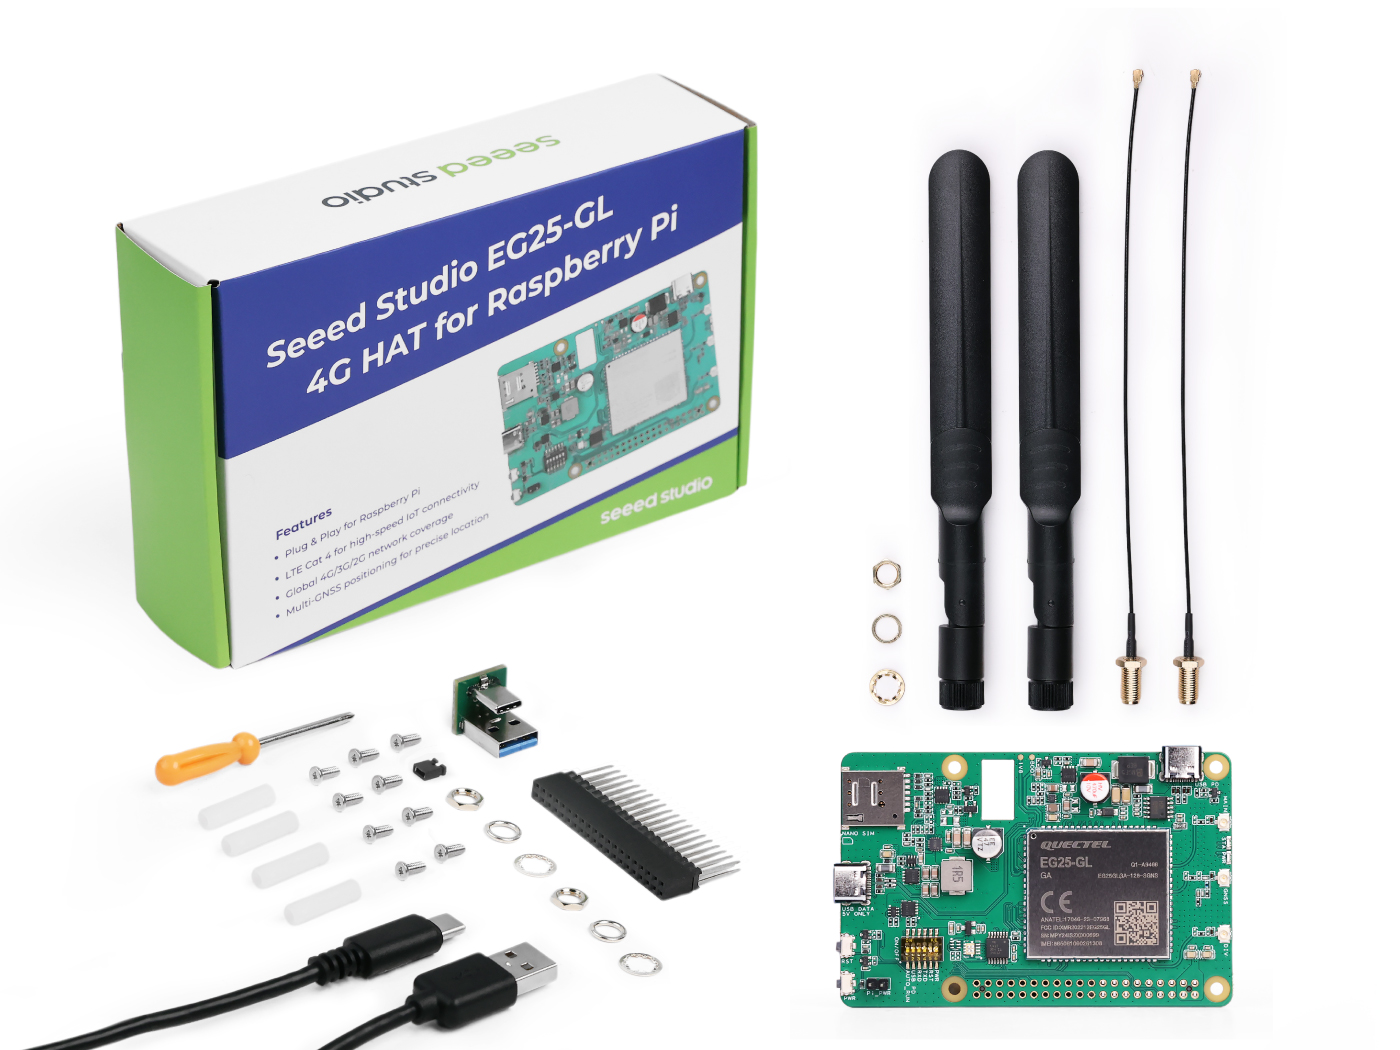
\includegraphics[width=0.5\linewidth,keepaspectratio]{media/image68.png}
  \caption{Módulo HAT 4G LTE con módem Quectel EG25-G sobre la Raspberry Pi.}
  \label{fig:hat-4g}
  \fuente{Adaptado de la hoja de datos del fabricante.}
\end{figure}

\paragraph{Viabilidad de conectividad 4G/LTE en Lima.} Las principales operadoras de Lima Metropolitana
ofrecen cobertura LTE prácticamente continua en zonas urbanas, donde se ubican las intersecciones objetivo,
lo que hace viable el enlace celular sin tender cableado dedicado. No obstante, pueden presentarse zonas de
sombra, saturación de celda en horas punta o cortes temporales del servicio. Por ello el diseño contempla
respaldos en cascada: el EG25-G realiza \textit{fallback} automático a 3G (WCDMA) y 2G (GSM/EDGE) ante
cobertura 4G limitada; el gabinete admite además un enlace Ethernet cuando la infraestructura local lo
permite; y, de forma determinante, ante la ausencia total de enlace el módulo continúa operando en modo
local: sigue sensando, estimando tráfico y generando recomendaciones acotadas, mientras el controlador
semafórico mantiene el plan seguro y la autoridad final. De este modo la conectividad mejora la
coordinación, pero su pérdida nunca compromete la operación de la intersección.

\subsection{Unidad de control y aceleración de inferencia de visión}\label{subsec:unidad-control}

La unidad de control debe ejecutar simultáneamente visión por computadora, algoritmos de decisión, gestión
de comunicaciones y control de los dispositivos electromecánicos. Se selecciona la \textbf{Raspberry Pi 5 de
16\,GB} como controlador principal. La Tabla~\ref{tab:control-units} compara las dos plataformas evaluadas.

\begin{table}[H]
  \centering
  \caption{Comparación técnica de las unidades de control evaluadas.}
  \label{tab:control-units}
  \footnotesize
  \begin{tabular}{@{}lll@{}}
    \toprule
    \textbf{Característica} & \textbf{Raspberry Pi 5 (16\,GB)} & \textbf{NVIDIA Jetson Nano}\\
    \midrule
    CPU & BCM2712 Cortex-A76 4 núcleos @ 2.4\,GHz & Cortex-A57 4 núcleos @ 1.43\,GHz\\
    RAM & 16\,GB LPDDR4X-4267 & 4\,GB LPDDR4\\
    GPU & VideoCore VII @ 800\,MHz & 128 núcleos Maxwell\\
    Aceleración IA & Coral TPU (4 TOPS) & GPU CUDA (472 GFLOPS)\\
    Interfaces de cámara & 2$\times$ MIPI CSI (4 carriles) & 1$\times$ MIPI CSI\\
    USB & 2$\times$ USB 3.0 + 2$\times$ USB 2.0 & 4$\times$ USB 3.0\\
    Ethernet & Gigabit + PoE+ & Gigabit\\
    Wi-Fi & 802.11ac doble banda & 802.11ac\\
    GPIO & 40 pines & 40 pines\\
    Alimentación & 5\,V/5\,A (25\,W) & 5\,V/4\,A (20\,W)\\
    \bottomrule
  \end{tabular}
  \fuente{Elaboración propia con datos de los fabricantes.}
\end{table}

La Raspberry Pi 5 supera al Jetson Nano en aspectos críticos para esta aplicación: su CPU Cortex-A76 a
2.4\,GHz ofrece un rendimiento por núcleo del orden de 75\,\% superior, sus 16\,GB de RAM frente a 4\,GB
permiten mantener varios modelos y buffers de video en memoria, y su puerto PCIe 2.0 x1 habilita expansión
con aceleradores externos. La aceleración de inferencia se delega al \textbf{Google Coral USB Accelerator},
basado en la Edge TPU, que alcanza 4\,TOPS con modelos cuantizados de 8 bits (TensorFlow Lite) consumiendo
solo 2--3\,W, liberando a la CPU para el resto de tareas del sistema.

\begin{figure}[H]
  \centering
  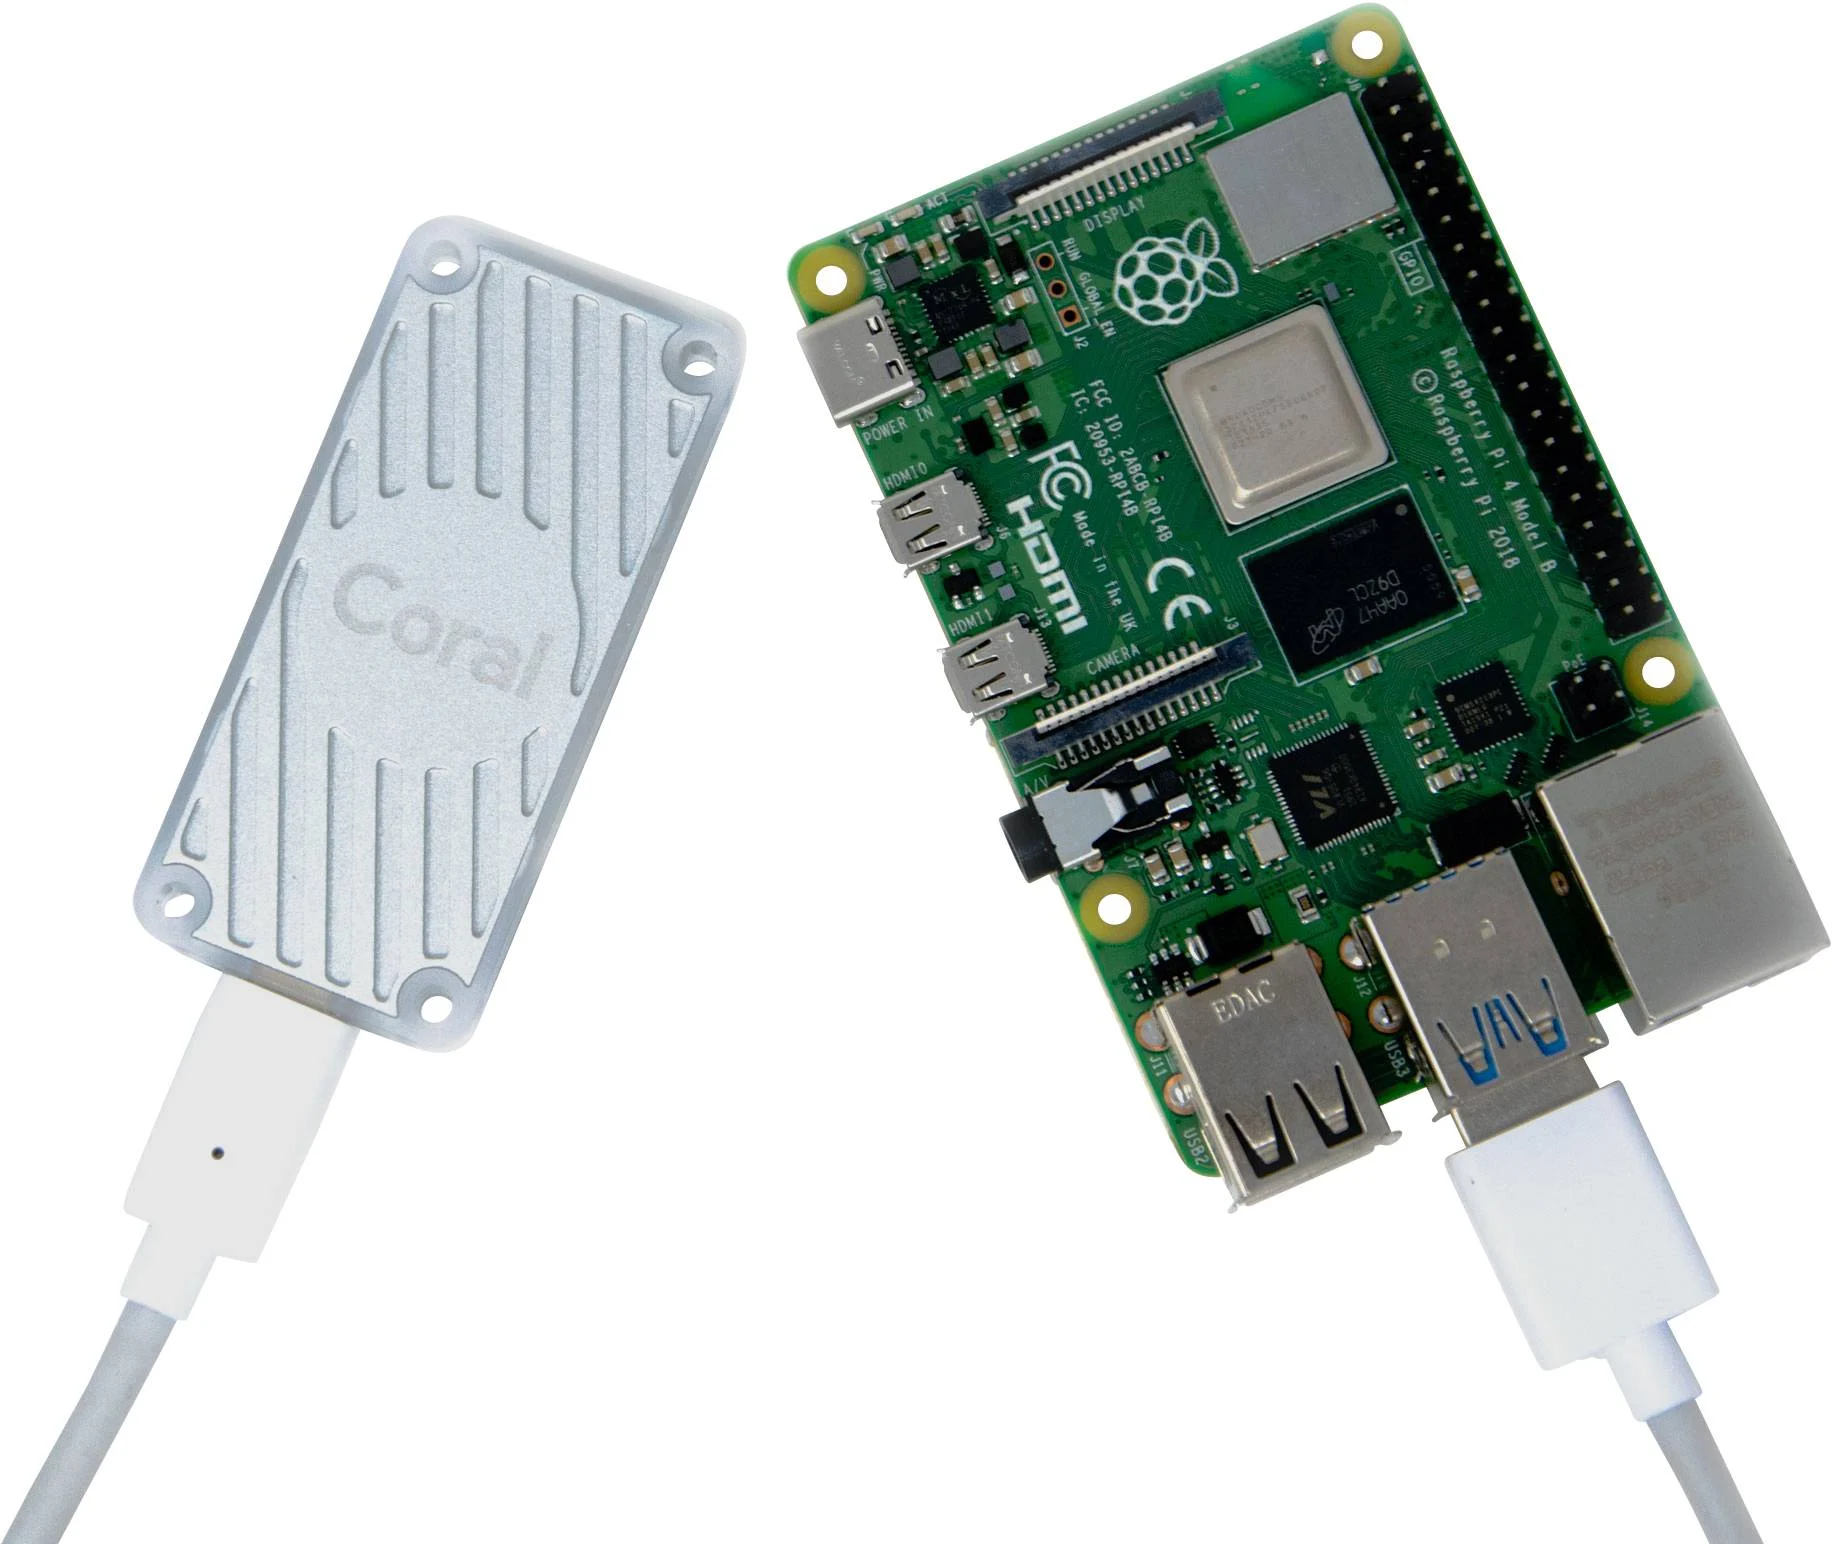
\includegraphics[width=0.5\linewidth,keepaspectratio]{media/image21.png}
  \caption{Conexión del acelerador Google Coral Edge TPU a la Raspberry Pi 5.}
  \label{fig:coral}
  \fuente{Adaptado de la documentación del fabricante.}
\end{figure}

\section{Dimensionamiento energético y protecciones}\label{sec:dimensionamiento}

Para garantizar un dimensionamiento adecuado y una operación estable se analiza el consumo de cada
componente a partir de las especificaciones de los fabricantes, en escenario de carga máxima. El cálculo se
estructura en etapas: consumo por componente, agregación por nivel de voltaje, aplicación del factor de
seguridad, selección de fuentes y convertidores, y finalmente la selección del UPS con su autonomía.

\subsection{Consumo por componente y por nivel de voltaje}

La Tabla~\ref{tab:consumo-componente} detalla el consumo por componente y la
Tabla~\ref{tab:consumo-voltaje} lo agrupa por nivel de voltaje de alimentación.

\begin{table}[H]
  \centering
  \caption{Consumo energético por componente.}
  \label{tab:consumo-componente}
  \footnotesize
  \begin{tabular}{@{}lcccl@{}}
    \toprule
    \textbf{Componente} & \textbf{V oper.} & \textbf{Corriente} & \textbf{Potencia (W)} & \textbf{Observaciones}\\
    \midrule
    Raspberry Pi 5 (16\,GB) & 5\,V DC & 5\,A & 25.0 & Carga máxima con periféricos\\
    Sensor DS18B20 & 5\,V DC & 0.0015\,A & 0.0075 & Corriente durante conversión\\
    Sensor WCS1600 & 5\,V DC & 0.02\,A & 0.1 & Operación normal\\
    Sensor URM06 & 12\,V DC & 0.05\,A & 0.6 & Detección continua\\
    Cámara DS-2CE57H0T-VPITF & 12\,V DC & 0.5\,A & 6.0 & Con IR encendido (máximo)\\
    Motor paso a paso NEMA 23 & 24\,V DC & 4.2\,A & 100.8 & Por fase, operación continua\\
    Driver DM542T & 24\,V DC & 0.3\,A & 7.2 & Standby\\
    HAT 4G LTE (EG25-G) & 5\,V DC & 0.6\,A & 3.0 & Transmisión activa\\
    Google Coral TPU & 5\,V DC & 0.6\,A & 3.0 & Inferencia activa\\
    Convertidor de nivel lógico & 5\,V DC & 0.01\,A & 0.05 & Bajo consumo\\
    ADC MCP3008 & 5\,V DC & 0.002\,A & 0.01 & Para sensor de corriente\\
    \bottomrule
  \end{tabular}
  \fuente{Elaboración propia con datos de los fabricantes.}
\end{table}

El consumo agrupado por voltaje se obtiene sumando los consumos individuales:
\[ P_{5\,\mathrm{V}} = 25 + 3 + 3 + 0.05 + 0.01 + 0.1 + 0.0075 = 31.1675\ \mathrm{W} \]
\[ P_{12\,\mathrm{V}} = 6 + 0.6 = 6.6\ \mathrm{W} \qquad P_{24\,\mathrm{V}} = 100.8 + 7.2 = 108\ \mathrm{W} \]

\begin{table}[H]
  \centering
  \caption{Consumo teórico de diseño por nivel de voltaje.}
  \label{tab:consumo-voltaje}
  \footnotesize
  \begin{tabular}{@{}lccc@{}}
    \toprule
    \textbf{Voltaje} & \textbf{Potencia (W)} & \textbf{Corriente (A)} & \textbf{\% del total}\\
    \midrule
    5\,V DC & 31.1675 & 6.23 & 21.4\,\%\\
    12\,V DC & 6.6 & 0.55 & 4.5\,\%\\
    24\,V DC & 108.0 & 4.5 & 74.1\,\%\\
    \textbf{TOTAL} & \textbf{145.7675} & --- & \textbf{100\,\%}\\
    \bottomrule
  \end{tabular}
  \fuente{Elaboración propia.}
\end{table}

La potencia total sin factor de seguridad es de aproximadamente 146\,W. Conforme al criterio de la norma de
controladores semafóricos NEMA Standards Publication TS 2-2021, se aplica un factor de seguridad del 25\,\%
para garantizar operación estable:
\[ 145.7675\ \mathrm{W} \times 1.25 = 182.21\ \mathrm{W} \]

\subsection{Convertidores DC-DC auxiliares}

Dado que el 74.1\,\% del consumo se concentra en 24\,V DC, la alimentación principal se centraliza en ese
bus y los voltajes secundarios (5\,V y 12\,V) se derivan con convertidores DC-DC de alta eficiencia, lo que
minimiza pérdidas y EMI. Los convertidores se dimensionan para operar al 80--90\,\% de su capacidad nominal,
prolongando su vida útil y mejorando la disipación térmica.

Para 12\,V DC se selecciona el \textbf{PULS CD5.121} (96\,W, eficiencia 88.2\,\%). Su potencia útil cubre
ampliamente la demanda de la línea:
\[ P_{\mathrm{salida},\,12} = 96\ \mathrm{W} \times 0.882 = 84.67\ \mathrm{W} \gg 6.6\ \mathrm{W} \]
suficiente para la cámara (6\,W) y el sensor URM06 (0.6\,W) con amplio margen térmico.

Para 5\,V DC se selecciona el \textbf{PULS CD5.051} (50\,W, 10\,A, eficiencia 81.5\,\%):
\[ P_{\mathrm{salida},\,5} = 50\ \mathrm{W} \times 0.815 = 40.75\ \mathrm{W} \]
frente a una demanda de 31.17\,W (6.23\,A), lo que deja un margen de 9.58\,W (\ensuremath{\approx}30.7\,\%) y
1.92\,A para transitorios y expansión ligera.

\begin{figure}[H]
  \centering
  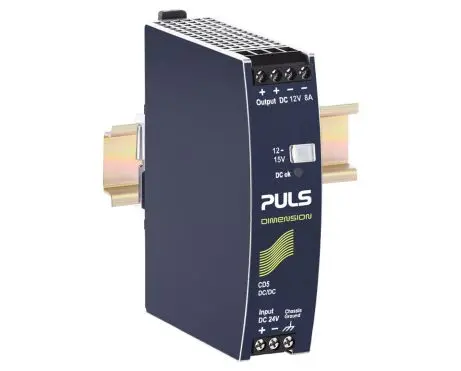
\includegraphics[width=0.45\linewidth,keepaspectratio]{media/image86.png}
  \caption{Convertidor DC-DC PULS CD5.121 (24\,V a 12\,V).}
  \label{fig:puls12}
  \fuente{Adaptado de la hoja de datos del fabricante.}
\end{figure}

\begin{figure}[H]
  \centering
  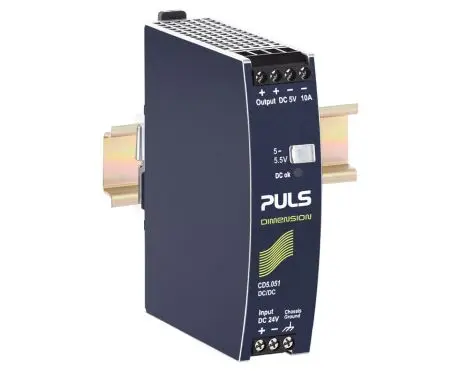
\includegraphics[width=0.45\linewidth,keepaspectratio]{media/image87.png}
  \caption{Convertidor DC-DC PULS CD5.051 (24\,V a 5\,V).}
  \label{fig:puls5}
  \fuente{Adaptado de la hoja de datos del fabricante.}
\end{figure}

Considerando las pérdidas de conversión, la potencia de entrada de los convertidores DC-DC desde el bus de
24\,V es:
\[ P_{\mathrm{entrada\ DC\text{-}DC}} = \frac{P_{5\,\mathrm{V}}}{\eta_{5}} + \frac{P_{12\,\mathrm{V}}}{\eta_{12}} = 56.86\ \mathrm{W} \]
y, sumada al consumo directo en 24\,V con su factor de seguridad, la potencia total requerida en ese bus es:
\[ P_{24\,\mathrm{V}} = 108\ \mathrm{W} \times 1.25 + 56.86\ \mathrm{W} = 191.86\ \mathrm{W} \]

\subsection{Fuente de alimentación conmutada (SMPS)}

Para alimentar el sistema desde la red AC 220\,V/60\,Hz se selecciona una SMPS de salida 24\,V DC que debe
superar la potencia de diseño (191.86\,W) con alta eficiencia. Se elige el modelo \textbf{S-360-24}
(360\,W, 15\,A):
\[ \mathrm{Margen} = \frac{360}{191.86} = 1.88 \qquad I_{24\,\mathrm{V}} = \frac{191.86}{24} = 8\ \mathrm{A} \]
La fuente opera a $191.86/360 = 53.3\,\%$ de su capacidad, dentro de la zona de eficiencia óptima, lo que
reduce el estrés térmico. Con eficiencia del 84\,\%, sus pérdidas son de unos 36.5\,W.

\begin{figure}[H]
  \centering
  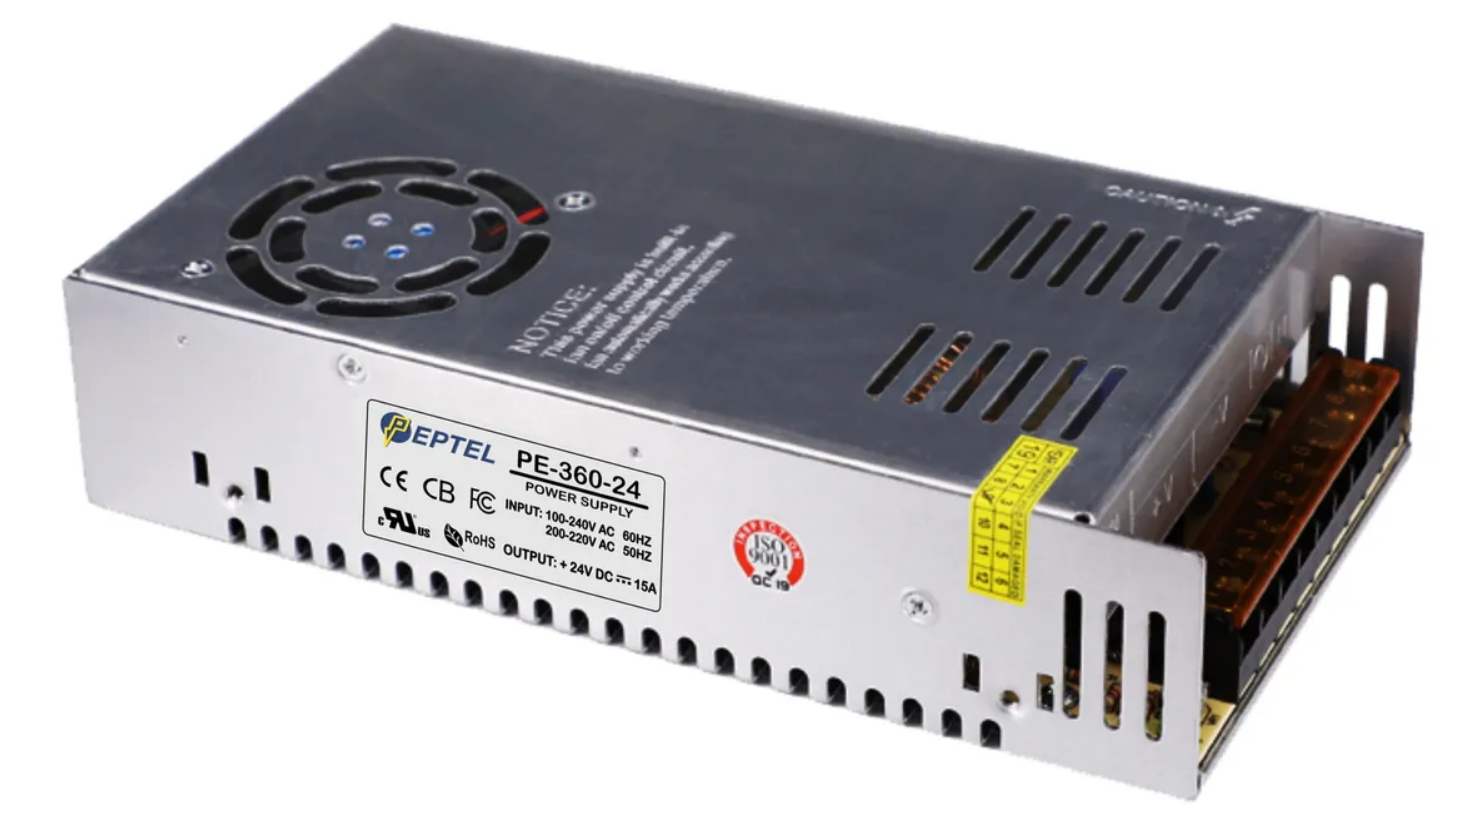
\includegraphics[width=0.5\linewidth,keepaspectratio]{media/image114.png}
  \caption{Fuente de alimentación conmutada AC/DC S-360-24 (360\,W, 24\,V, 15\,A).}
  \label{fig:smps}
  \fuente{Adaptado de la hoja de datos del fabricante.}
\end{figure}

La corriente de entrada desde la red, considerando una eficiencia del 85\,\%, es:
\[ P_{\mathrm{AC}} = \frac{191.86\ \mathrm{W}}{0.85} = 228.4\ \mathrm{W} \qquad I_{\mathrm{AC}} = \frac{228.4}{220} = 1.04\ \mathrm{A} \]
Este valor define los umbrales de monitoreo del sensor de corriente WCS1600: $\pm20\,\%$ alrededor de
1.04\,A, es decir, el rango [0.83\,A, 1.25\,A].

\subsection{Sistema de alimentación ininterrumpida (UPS)}

Para mantener la continuidad durante cortes de red se ubica un \textbf{UPS} aguas arriba de la SMPS. Con un
banco de baterías AGM de $2\times12$\,V/12\,Ah:
\[ \mathrm{Capacidad}_{\mathrm{bater\acute{i}a}} = 2 \times 12\ \mathrm{V} \times 12\ \mathrm{Ah} = 288\ \mathrm{Wh} \]
\[ P_{\mathrm{disponible}} = 288\ \mathrm{Wh} \times 0.95 = 273.6\ \mathrm{Wh} \]
\[ t_{\mathrm{autonom\acute{i}a}} = \frac{273.6\ \mathrm{Wh}}{228.4\ \mathrm{W}} \approx 72\ \mathrm{min} \]
El modelo seleccionado (APC SMT1500IC, 1000\,W) ofrece un margen de $1000/228.4 = 4.38$ veces la demanda del
sistema, con salida de onda senoidal pura, lo que facilita expansiones y reduce el estrés térmico de las
baterías. La autonomía de 72\,min es suficiente para un registro y apagado controlados. Por su formato de
torre, el UPS se instala en la base del poste y alimenta el gabinete a través de la SMPS; en el rack en altura
solo se aloja la interfaz de baterías y la gestión del respaldo, lo que evita cargar el conjunto superior con
su masa.

\begin{figure}[H]
  \centering
  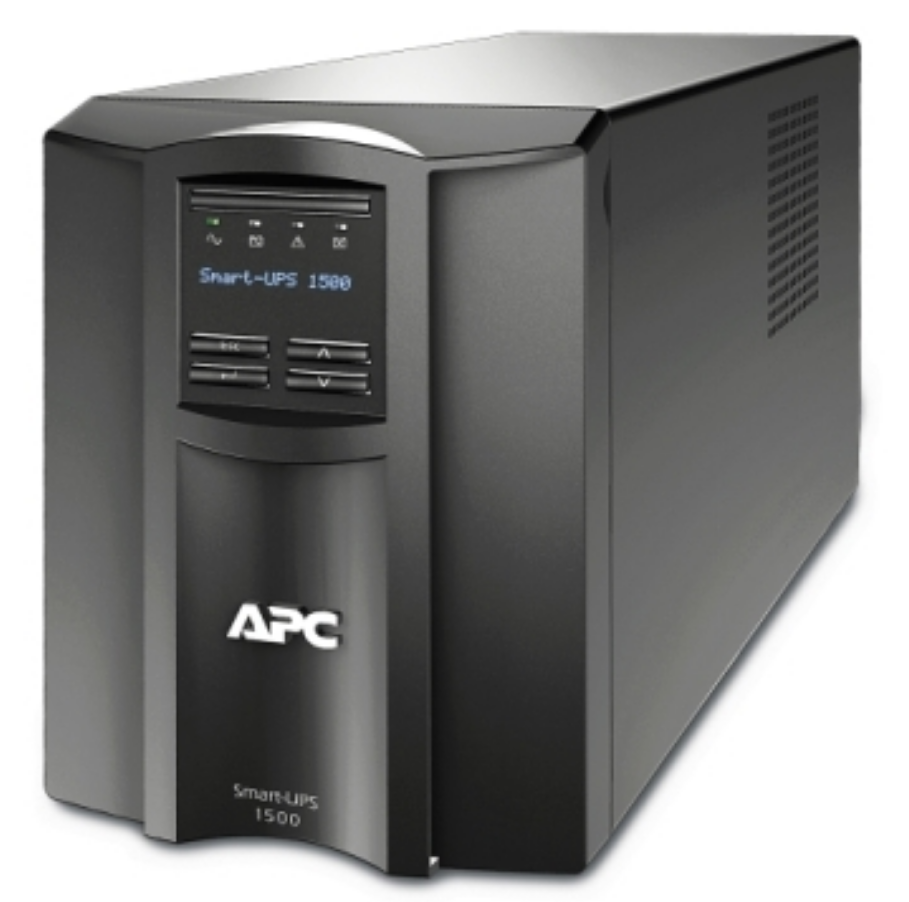
\includegraphics[width=0.4\linewidth,keepaspectratio]{media/image6.png}
  \caption{Sistema de alimentación ininterrumpida (UPS) de respaldo.}
  \label{fig:ups}
  \fuente{Adaptado de la documentación del fabricante.}
\end{figure}

\subsection{Protecciones eléctricas coordinadas}

La protección de la línea AC combina cuatro dispositivos coordinados. El interruptor termomagnético
\textbf{Schneider C60N-C6} protege contra sobrecargas y cortocircuitos; aplicando el criterio NEC/IEC,
$I_{\mathrm{breaker}} \geq 1.25 \times 1.04\ \mathrm{A} = 1.3\ \mathrm{A}$, por lo que un breaker de 6\,A
curva C aporta un factor de $6/1.04 = 5.77$ y tolera los picos moderados de cargas electrónicas. El
dispositivo de protección contra sobretensiones (DPS) \textbf{Phoenix Contact VAL-MS 230} deriva a tierra
las sobretensiones transitorias (respuesta $<$100\,ns, nivel de protección 1.5\,kV) mediante varistores,
protegido a su vez por el fusible interno \textbf{F-MS 12 ST}. El interruptor diferencial (RCD)
\textbf{Schneider ID K 25A 30mA} protege al personal de mantenimiento contra fugas a tierra: con un umbral
de 30\,mA y disparo $\leq$30\,ms, mantiene un margen de 4.33 veces respecto al límite de fibrilación
ventricular.

\begin{figure}[H]
  \centering
  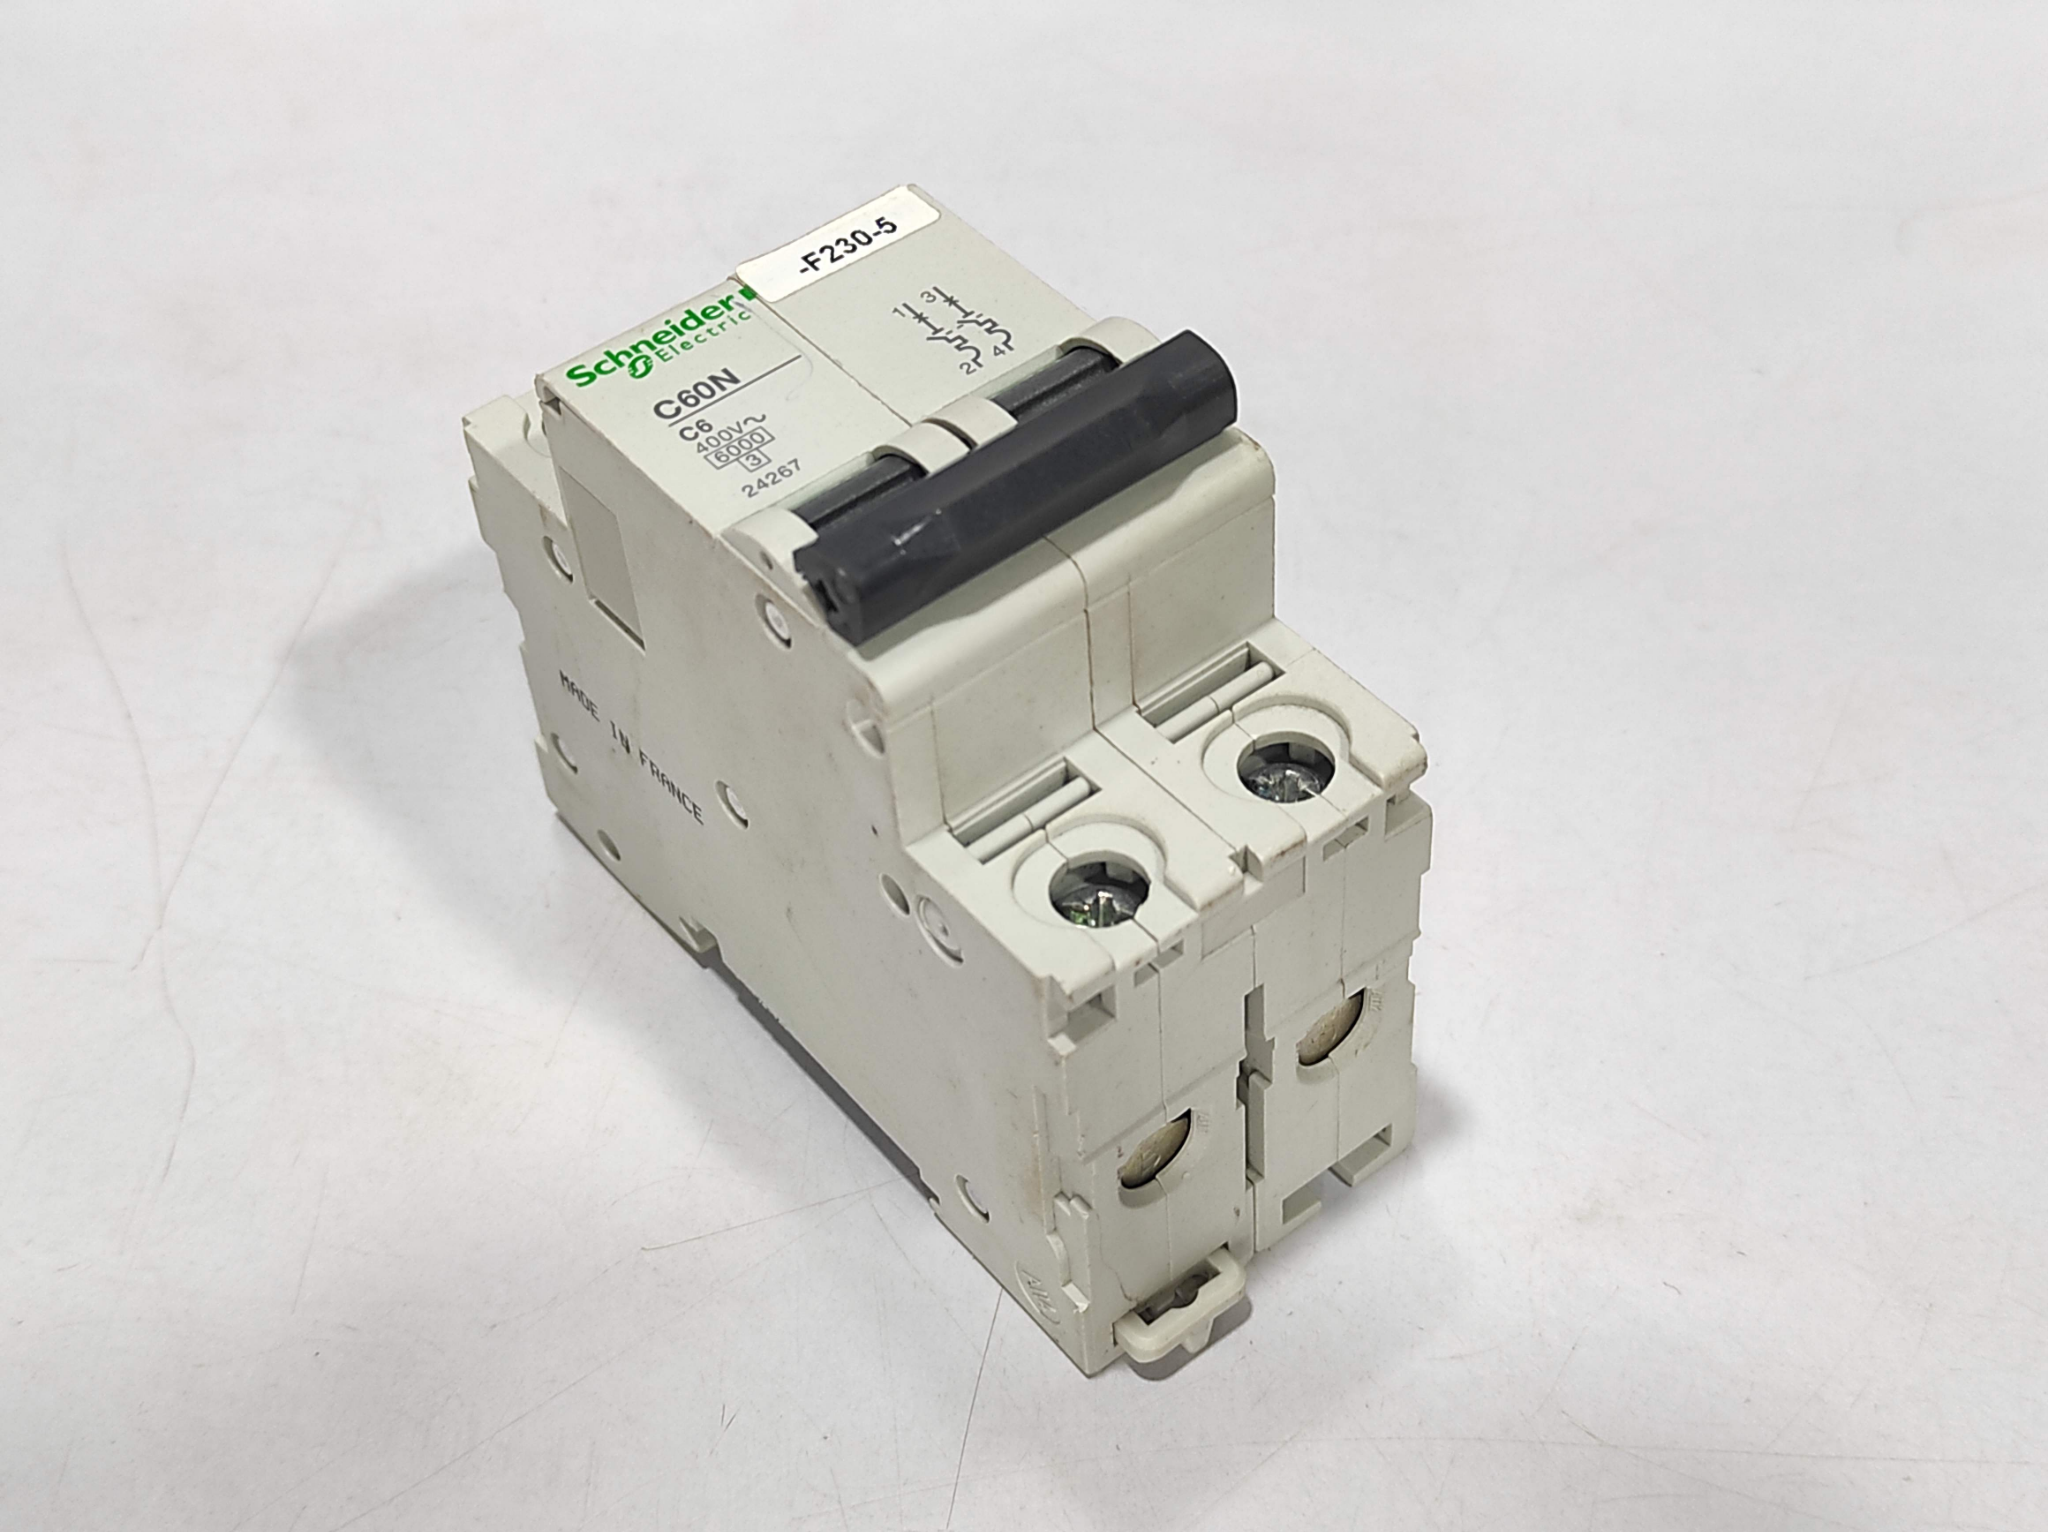
\includegraphics[width=0.5\linewidth,keepaspectratio]{media/image72.png}
  \caption{Interruptor termomagnético Schneider Electric C60N-C6.}
  \label{fig:breaker}
  \fuente{Adaptado de la hoja de datos del fabricante.}
\end{figure}

\begin{figure}[H]
  \centering
  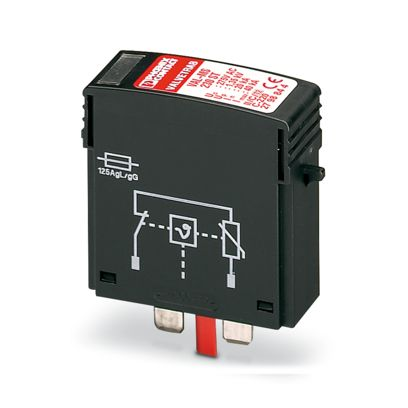
\includegraphics[width=0.5\linewidth,keepaspectratio]{media/image136.png}
  \caption{Dispositivo de protección contra sobretensiones Phoenix Contact VAL-MS 230 con fusible F-MS 12 ST.}
  \label{fig:dps}
  \fuente{Adaptado de la hoja de datos del fabricante.}
\end{figure}

\begin{figure}[H]
  \centering
  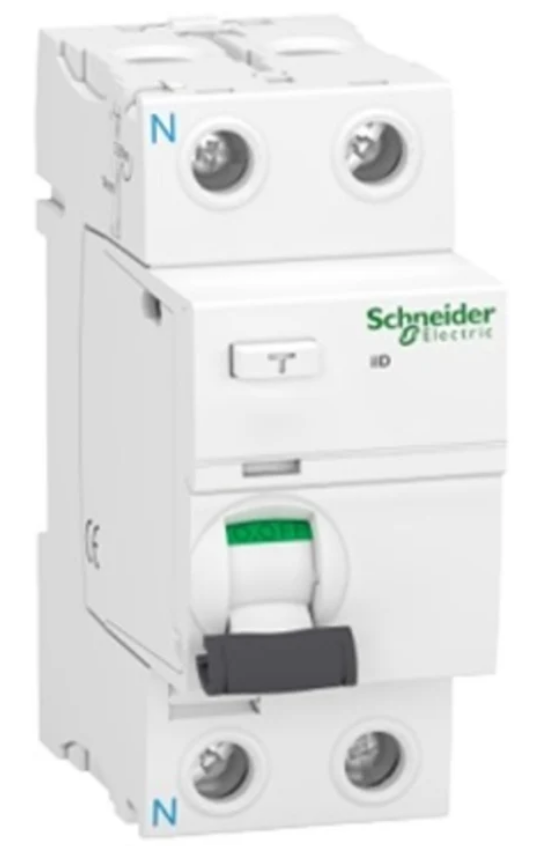
\includegraphics[width=0.5\linewidth,keepaspectratio]{media/image35.png}
  \caption{Interruptor diferencial Schneider Electric ID K 25A 30mA.}
  \label{fig:rcd}
  \fuente{Adaptado de la hoja de datos del fabricante.}
\end{figure}

El orden de instalación responde a la coordinación selectiva de las normas IEC 60364-5-53 y NEC Article 285,
ilustrada en la Figura~\ref{fig:proteccion-circuito}. El breaker se ubica primero como protección primaria,
limitando la corriente antes de los dispositivos aguas abajo y protegiendo al RCD de corrientes destructivas.
El RCD se instala a continuación para detectar fugas a tierra una vez asegurada la protección contra fallas
catastróficas. Finalmente, el DPS se ubica aguas abajo del RCD, de modo que las corrientes de descarga
(hasta 10\,kA en pulsos 8/20\,\ensuremath{\mu}s) no sean interpretadas como fugas y provoquen disparos
intempestivos; ante una falla del varistor por fin de vida útil, el breaker aguas arriba y el fusible interno
del DPS interrumpen el circuito de forma escalonada. La Tabla~\ref{tab:lista-alimentacion} resume la
selección del sistema de alimentación y protecciones.

\begin{figure}[H]
  \centering
  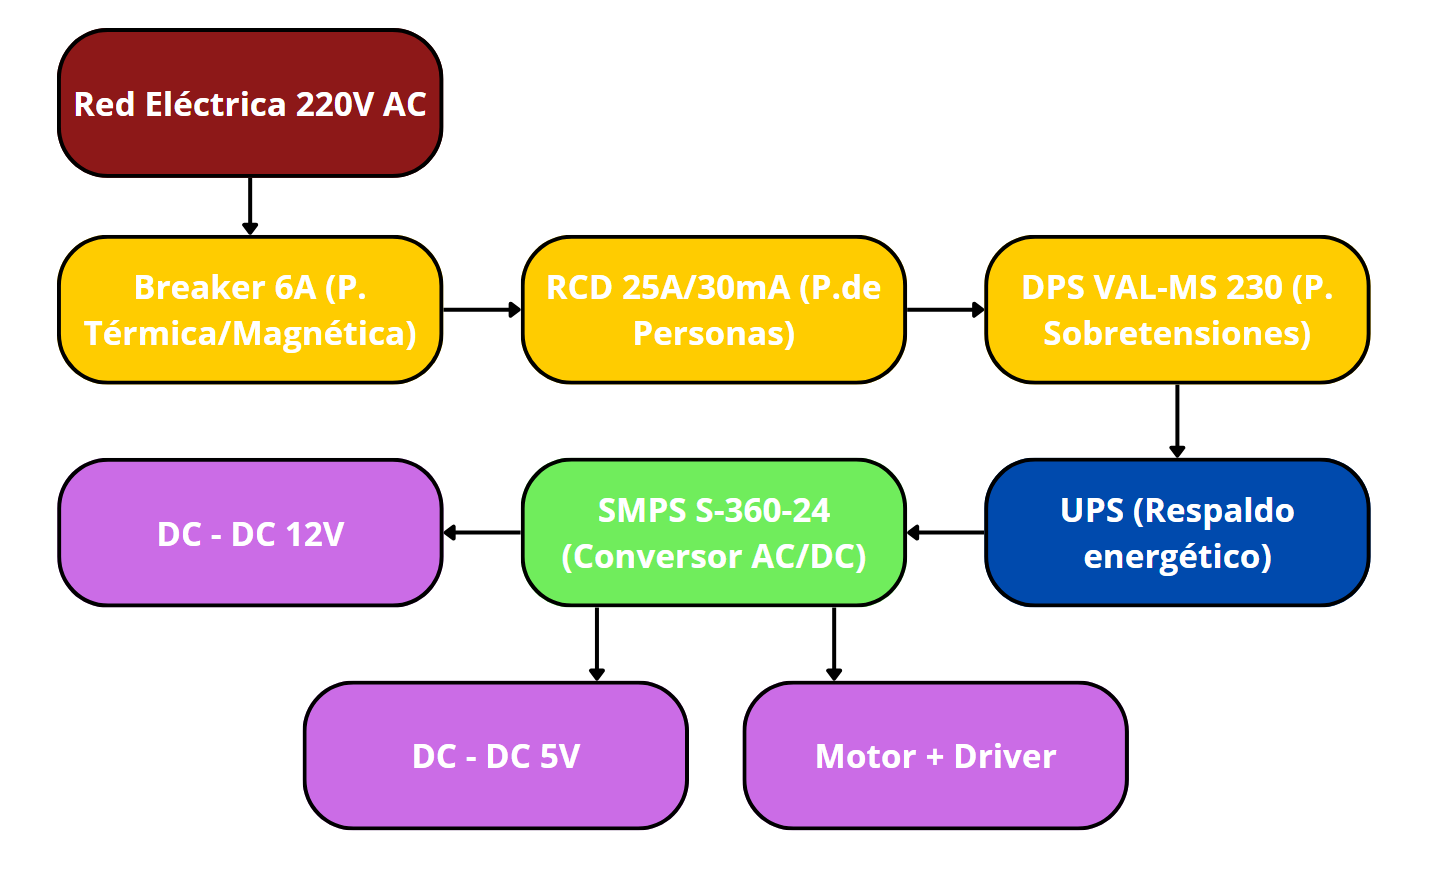
\includegraphics[width=0.75\linewidth,keepaspectratio]{media/image40.png}
  \caption{Circuito de protecciones eléctricas coordinadas (breaker, RCD y DPS).}
  \label{fig:proteccion-circuito}
  \fuente{Elaboración propia.}
\end{figure}

\begin{table}[H]
  \centering
  \caption{Lista de componentes del sistema de alimentación y protecciones.}
  \label{tab:lista-alimentacion}
  \footnotesize
  \begin{tabular}{@{}p{2.6cm}p{3.4cm}p{7.5cm}@{}}
    \toprule
    \textbf{Componente} & \textbf{Modelo seleccionado} & \textbf{Justificación técnica}\\
    \midrule
    Breaker & Schneider C60N-C6 & Corriente nominal 6\,A $>$ 1.3\,A requerida; curva C\\
    DPS & Phoenix VAL-MS 230 & Sobretensiones; respuesta $<$100\,ns; fuga $<$10\,\ensuremath{\mu}A\\
    RCD & Schneider ID K 25A 30mA & Protección de personas; sensibilidad 30\,mA; disparo $\leq$30\,ms\\
    UPS & APC SMT1500IC & 1000\,W $>$ 228.4\,W (factor 4.38); autonomía 72\,min; onda senoidal pura\\
    SMPS principal & S-360-24 & 360\,W $>$ 191.86\,W (factor 1.88); eficiencia $>$84\,\%; operación al 53.3\,\%\\
    DC-DC 5\,V & PULS CD5.051 & 40.75\,W útiles $>$ 31.17\,W requeridos; margen 30.7\,\%\\
    DC-DC 12\,V & PULS CD5.121 & 84.67\,W útiles $>$ 6.6\,W requeridos; eficiencia 88.2\,\%\\
    \bottomrule
  \end{tabular}
  \fuente{Elaboración propia.}
\end{table}

\section{Costos del módulo electrónico}\label{sec:costos-electronico}

Como insumo para el análisis CAPEX del Capítulo~\ref{cap:analisis-economico}, la
Tabla~\ref{tab:costos-electronica} presenta una estimación de costos por componente del módulo electrónico.
Los valores corresponden a órdenes de magnitud referenciales del mercado peruano (soles, 2025--2026) y no a
cotizaciones formales; se incluyen para dimensionar la inversión y pueden variar según proveedor, importación
y tipo de cambio. No se incluyen aquí el gabinete ni los elementos mecánicos, que se costean en el
Capítulo~\ref{cap:diseno-mecanico}.

\begin{table}[H]
  \centering
  \caption{Estimación de costos por componente del módulo electrónico (valores referenciales).}
  \label{tab:costos-electronica}
  \footnotesize
  \begin{tabular}{@{}p{7.5cm}cr@{}}
    \toprule
    \textbf{Componente} & \textbf{Cant.} & \textbf{Costo aprox. (S/)}\\
    \midrule
    Raspberry Pi 5 (16\,GB) & 1 & 650\\
    Google Coral USB Accelerator & 1 & 450\\
    HAT 4G LTE (Quectel EG25-G) & 1 & 380\\
    Cámara domo Hikvision DS-2CE57H0T-VPITF & 1 & 180\\
    Convertidor de video 4-en-1 a USB & 1 & 90\\
    Sensor de temperatura DS18B20 & 1 & 15\\
    Sensor de corriente WCS1600 + ADC MCP3008 & 1 & 55\\
    Sensor ultrasónico URM06 & 1 & 180\\
    Motor paso a paso NEMA 23 & 1 & 160\\
    Driver DM542T & 1 & 120\\
    Convertidor de nivel lógico TXS0108E & 1 & 15\\
    Fuente conmutada S-360-24 & 1 & 180\\
    Convertidor DC-DC PULS CD5.051 (5\,V) & 1 & 320\\
    Convertidor DC-DC PULS CD5.121 (12\,V) & 1 & 380\\
    UPS APC SMT1500IC & 1 & 2\,280\\
    Breaker Schneider C60N-C6 & 1 & 80\\
    RCD Schneider ID K 25A 30mA & 1 & 220\\
    DPS Phoenix VAL-MS 230 + fusible F-MS 12 ST & 1 & 410\\
    PCBs personalizadas, conectores y cableado & 1 & 400\\
    \midrule
    \textbf{Total estimado del módulo electrónico} & & \textbf{$\approx$ 6\,565}\\
    \bottomrule
  \end{tabular}
  \fuente{Elaboración propia; precios referenciales del mercado peruano (2025--2026).}
\end{table}

El UPS y los convertidores DC-DC industriales PULS concentran buena parte del costo, lo que sugiere que en
una eventual optimización de CAPEX son los rubros con mayor sensibilidad. El detalle de este análisis se
retoma en el Capítulo~\ref{cap:analisis-economico}.

\section{Diagramas esquemáticos}\label{sec:esquematicos}

Los diagramas presentados en esta sección son \textbf{esquemáticos de diseño}, orientados a documentar la
arquitectura eléctrica, la conexión entre subsistemas y el dimensionamiento de protecciones y filtrado. No
constituyen archivos de manufactura: no se ha ejecutado una verificación de reglas de diseño (DRC) ni la
generación de \textit{Gerbers} para fabricación, etapas que corresponderían a una fase posterior de
ingeniería de producción. La disposición física de estos elementos en el gabinete (distribución por zonas
funcionales en rack de 19", separación electromagnética y térmica, y cableado) es contenido mecánico y se
desarrolla en el Capítulo~\ref{cap:diseno-mecanico}.

\subsection{Sistema de alimentación y protecciones}

La Figura~\ref{fig:esq-alimentacion} representa la arquitectura completa de alimentación, desde la red AC
hasta las cargas DC. La entrada de 220\,V AC/60\,Hz atraviesa el breaker C60N-C6, el DPS VAL-MS 230 y el RCD
ID K 25A/30mA según la coordinación descrita; el UPS de 1500\,VA/1000\,W aporta el respaldo y alimenta la
SMPS S-360-24, que genera el bus principal de 24\,V DC. Desde ese bus se derivan tres líneas: una directa al
motor NEMA 23 y su driver DM542T, y dos hacia los convertidores PULS CD5.121 (12\,V para cámara y URM06) y
CD5.051 (5\,V para Raspberry Pi, HAT 4G LTE y demás cargas de bajo consumo).

\begin{figure}[H]
  \centering
  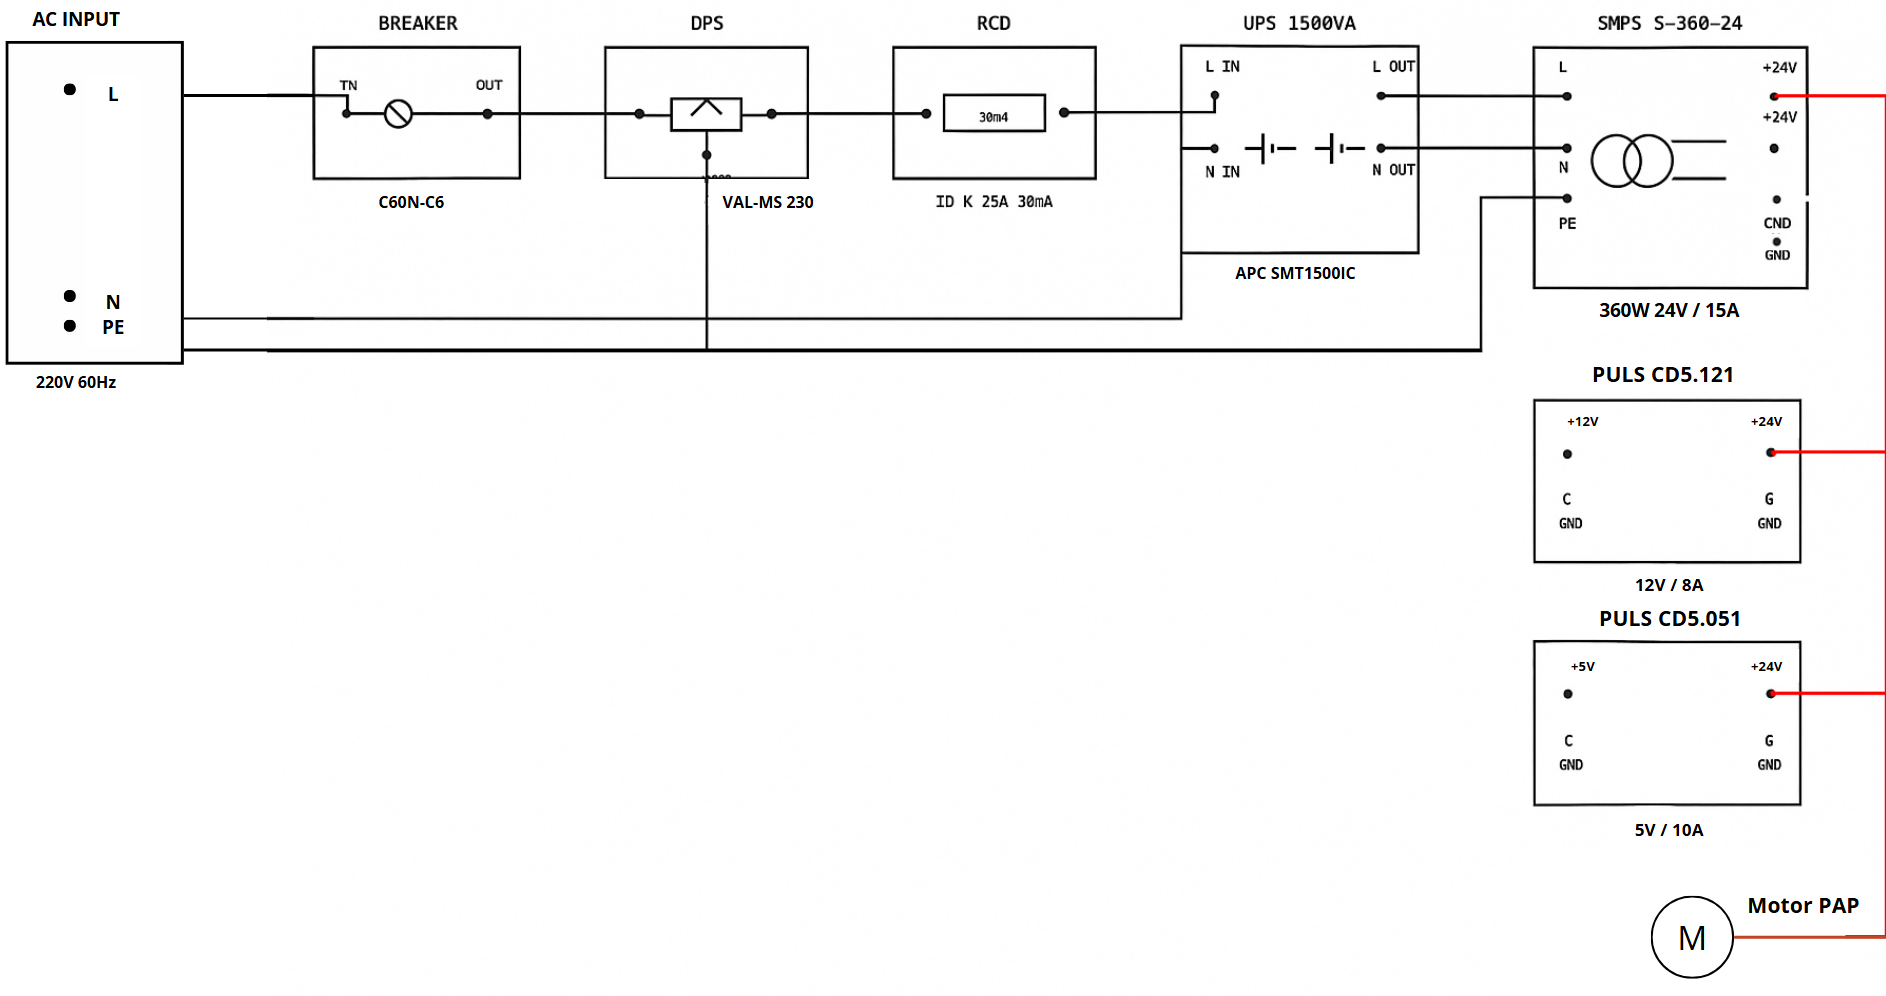
\includegraphics[width=0.85\linewidth,keepaspectratio]{media/image117.png}
  \caption{Esquemático del sistema de alimentación y protecciones.}
  \label{fig:esq-alimentacion}
  \fuente{Elaboración propia.}
\end{figure}

\subsection{PCB de distribución de alimentación}

La PCB de distribución implementa una topología en estrella con filtrado multicapa. El esquemático de 5\,V
(Figura~\ref{fig:esq-5v}) incorpora protección de entrada mediante diodo TVS bidireccional P6KE6.8CA (600\,W
pico) y fusible de 10\,A con margen sobre la corriente máxima de 6.23\,A. El banco de filtrado combina
capacitores electrolíticos de 1000\,\ensuremath{\mu}F y 470\,\ensuremath{\mu}F para baja frecuencia y
cerámicos de 1\,\ensuremath{\mu}F y 0.1\,\ensuremath{\mu}F para alta frecuencia, con un inductor
AIAP-03-121K de 120\,\ensuremath{\mu}H que forma un filtro LC (corte $\approx$46\,Hz) y atenúa el rizado del
convertidor a menos de 10\,mVpp. Cada salida incorpora capacitores localizados (470\,\ensuremath{\mu}F para
la Raspberry Pi, 100\,\ensuremath{\mu}F para el HAT 4G LTE). El circuito de 12\,V
(Figura~\ref{fig:esq-12v}) usa arquitectura análoga con TVS unidireccional SMAJ12A (400\,W), fusible de 5\,A
y un \textit{ferrite bead} BLM21PG121SN1D en lugar del inductor, optimizando la supresión de EMI generado por
la cámara.

\begin{figure}[H]
  \centering
  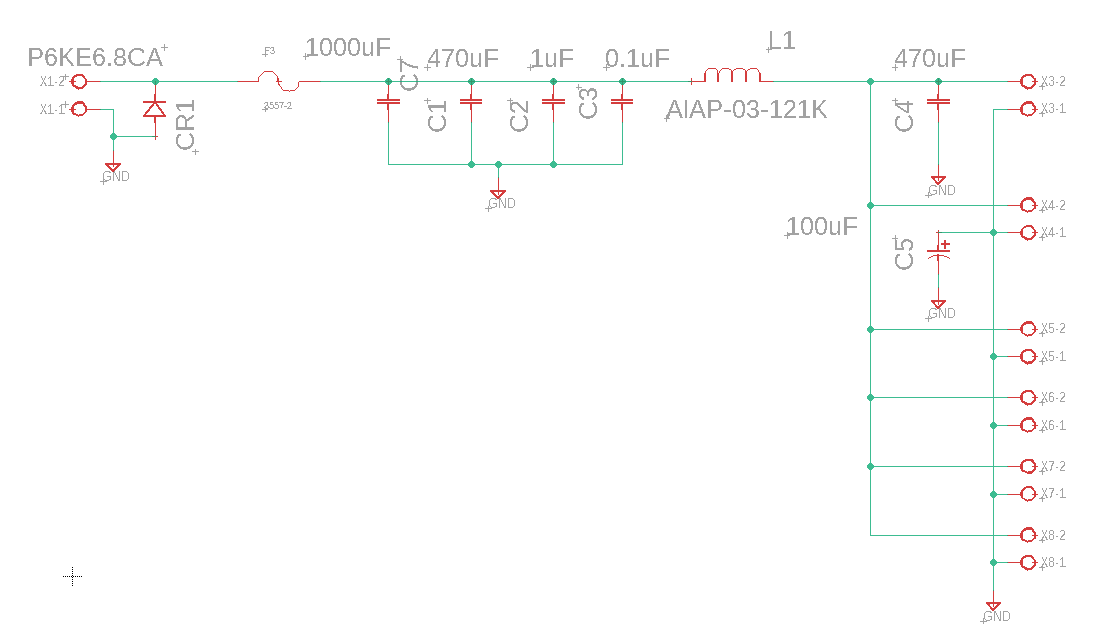
\includegraphics[width=0.8\linewidth,keepaspectratio]{media/image77.png}
  \caption{Esquemático de la línea de distribución de 5\,V.}
  \label{fig:esq-5v}
  \fuente{Elaboración propia.}
\end{figure}

\begin{figure}[H]
  \centering
  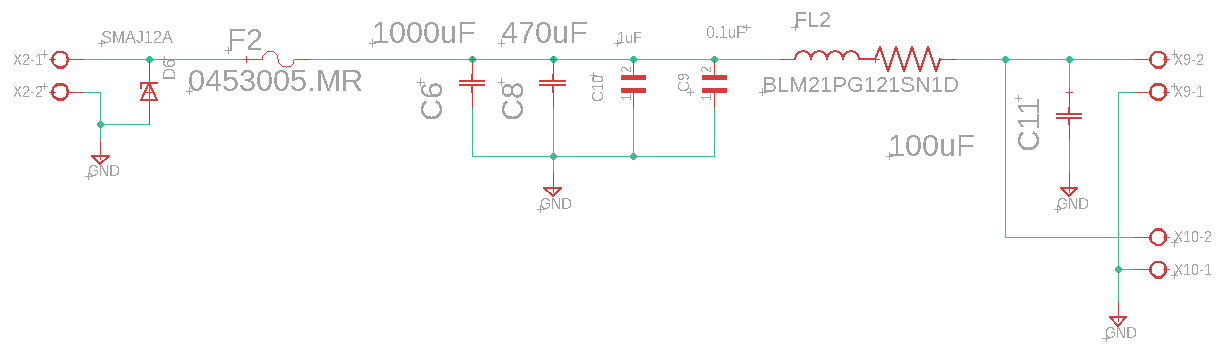
\includegraphics[width=0.8\linewidth,keepaspectratio]{media/image69.png}
  \caption{Esquemático de la línea de distribución de 12\,V.}
  \label{fig:esq-12v}
  \fuente{Elaboración propia.}
\end{figure}

La PCB de distribución (Figura~\ref{fig:pcb-distribucion}) se diseña en dos capas con cobre de 2\,oz
(70\,\ensuremath{\mu}m), lo que duplica la sección del conductor respecto al estándar de 1\,oz y mejora la
disipación térmica. Las pistas de 5\,V usan 2\,mm de ancho para 6.5\,A con elevación térmica $<$15\,°C, y las
de 12\,V usan 1.5\,mm para 1.5\,A con margen holgado. La disposición sigue un flujo direccional con las
entradas a la izquierda, los elementos de protección y los electrolíticos en la zona central, y los
capacitores cerámicos de desacoplo junto a cada conector de salida; las vías a tierra se distribuyen cada
10--15\,mm para reducir la impedancia en alta frecuencia.

\begin{figure}[H]
  \centering
  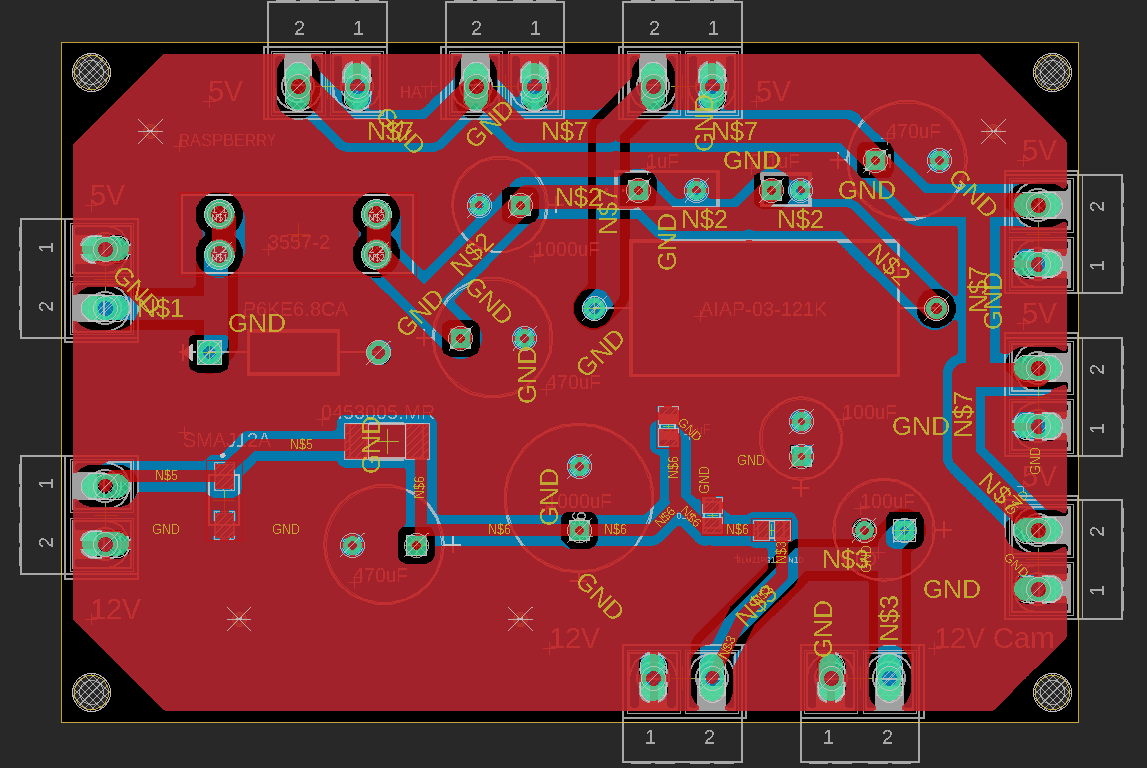
\includegraphics[width=0.8\linewidth,keepaspectratio]{media/image8.png}
  \caption{PCB de distribución de alimentación (diseño, sin verificación de manufactura).}
  \label{fig:pcb-distribucion}
  \fuente{Elaboración propia.}
\end{figure}

\subsection{PCB del controlador semafórico}

El esquemático de la PCB controladora (Figura~\ref{fig:esq-controlador}) integra las interfaces que conectan
sensores, actuadores y módulos periféricos a la Raspberry Pi 5, asegurando la compatibilidad de voltajes
entre los 5\,V de los periféricos y los 3.3\,V de los GPIO. El sensor de temperatura se conecta al GPIO 4 con
una resistencia pull-up de 4.7\,k\ensuremath{\Omega} para estabilizar la comunicación OneWire; el sensor de
corriente se digitaliza con el ADC MCP3008 por bus SPI (GPIO 8, 9, 10 y 11). El convertidor de nivel lógico
adapta las señales del sensor URM06 (GPIO 14 y 15) y del driver DM542T (DIR, PUL y ENA en los GPIO 17, 22 y
27). La cámara se conecta al puerto USB 2.0, reservando los USB 3.0 para el Coral y el HAT 4G LTE; todas las
tierras se unifican en un plano de GND común para minimizar bucles de tierra. La placa fabricada se muestra
en la Figura~\ref{fig:pcb-controlador}.

\begin{figure}[H]
  \centering
  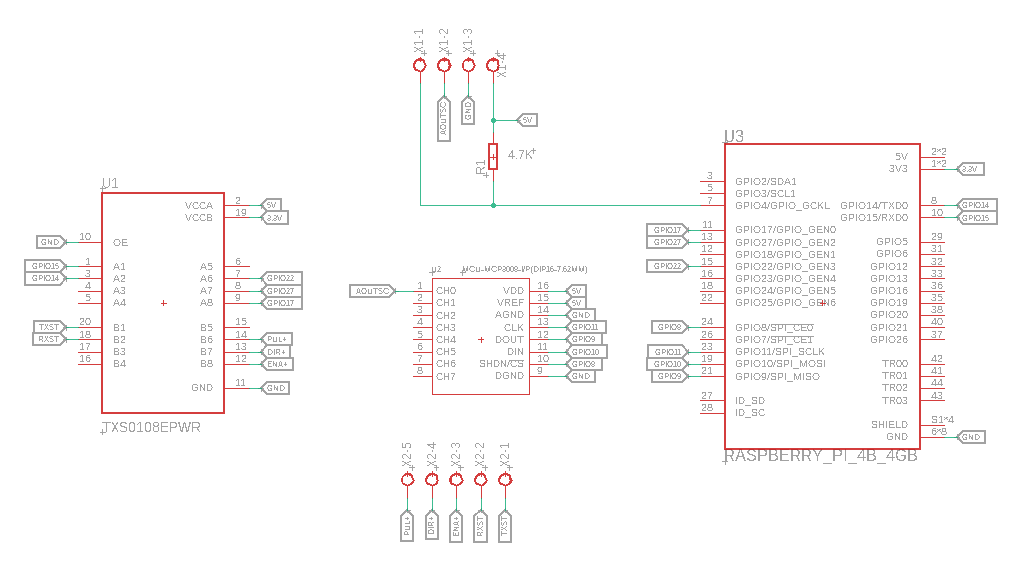
\includegraphics[width=0.8\linewidth,keepaspectratio]{media/image97.png}
  \caption{Esquemático de la PCB del controlador semafórico.}
  \label{fig:esq-controlador}
  \fuente{Elaboración propia.}
\end{figure}

\begin{figure}[H]
  \centering
  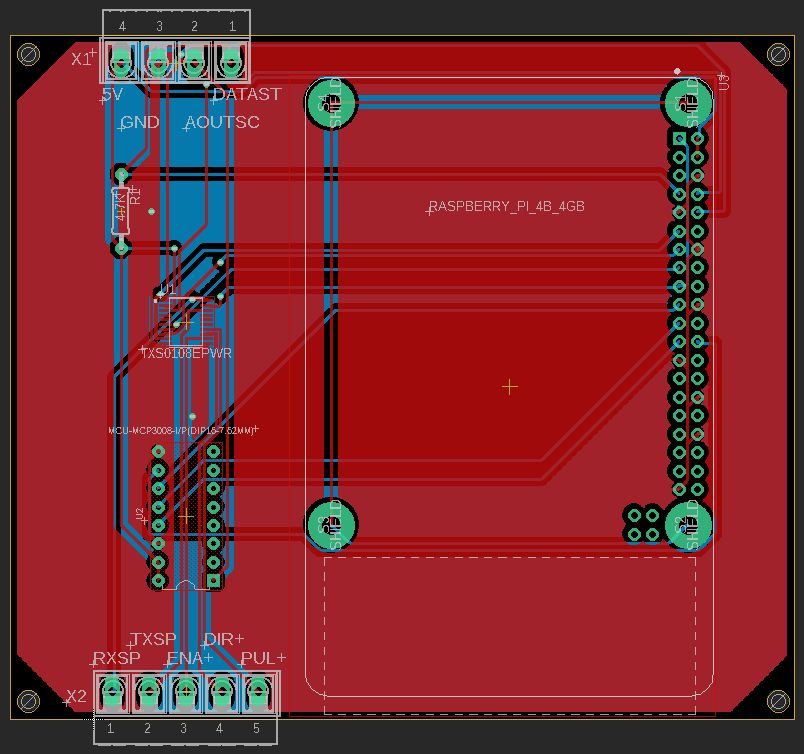
\includegraphics[width=0.8\linewidth,keepaspectratio]{media/image11.png}
  \caption{PCB del controlador semafórico (diseño, sin verificación de manufactura).}
  \label{fig:pcb-controlador}
  \fuente{Elaboración propia.}
\end{figure}
